% Options for packages loaded elsewhere
\PassOptionsToPackage{unicode}{hyperref}
\PassOptionsToPackage{hyphens}{url}
%
\documentclass[
]{book}
\usepackage{amsmath,amssymb}
\usepackage{lmodern}
\usepackage{iftex}
\ifPDFTeX
  \usepackage[T1]{fontenc}
  \usepackage[utf8]{inputenc}
  \usepackage{textcomp} % provide euro and other symbols
\else % if luatex or xetex
  \usepackage{unicode-math}
  \defaultfontfeatures{Scale=MatchLowercase}
  \defaultfontfeatures[\rmfamily]{Ligatures=TeX,Scale=1}
\fi
% Use upquote if available, for straight quotes in verbatim environments
\IfFileExists{upquote.sty}{\usepackage{upquote}}{}
\IfFileExists{microtype.sty}{% use microtype if available
  \usepackage[]{microtype}
  \UseMicrotypeSet[protrusion]{basicmath} % disable protrusion for tt fonts
}{}
\makeatletter
\@ifundefined{KOMAClassName}{% if non-KOMA class
  \IfFileExists{parskip.sty}{%
    \usepackage{parskip}
  }{% else
    \setlength{\parindent}{0pt}
    \setlength{\parskip}{6pt plus 2pt minus 1pt}}
}{% if KOMA class
  \KOMAoptions{parskip=half}}
\makeatother
\usepackage{xcolor}
\usepackage{longtable,booktabs,array}
\usepackage{calc} % for calculating minipage widths
% Correct order of tables after \paragraph or \subparagraph
\usepackage{etoolbox}
\makeatletter
\patchcmd\longtable{\par}{\if@noskipsec\mbox{}\fi\par}{}{}
\makeatother
% Allow footnotes in longtable head/foot
\IfFileExists{footnotehyper.sty}{\usepackage{footnotehyper}}{\usepackage{footnote}}
\makesavenoteenv{longtable}
\usepackage{graphicx}
\makeatletter
\def\maxwidth{\ifdim\Gin@nat@width>\linewidth\linewidth\else\Gin@nat@width\fi}
\def\maxheight{\ifdim\Gin@nat@height>\textheight\textheight\else\Gin@nat@height\fi}
\makeatother
% Scale images if necessary, so that they will not overflow the page
% margins by default, and it is still possible to overwrite the defaults
% using explicit options in \includegraphics[width, height, ...]{}
\setkeys{Gin}{width=\maxwidth,height=\maxheight,keepaspectratio}
% Set default figure placement to htbp
\makeatletter
\def\fps@figure{htbp}
\makeatother
\setlength{\emergencystretch}{3em} % prevent overfull lines
\providecommand{\tightlist}{%
  \setlength{\itemsep}{0pt}\setlength{\parskip}{0pt}}
\setcounter{secnumdepth}{5}
\usepackage{booktabs}
\usepackage{color}
\usepackage{tcolorbox}
\usepackage{float}
\graphicspath{ {images/} }

\newenvironment{rmdremind}
  {\begin{tcolorbox}[width=\textwidth, 
                     colback = {white}, 
                     title = {\textbf{Remember}}, 
                     colbacktitle = lightgray,
                     coltitle = black]
  \begin{includegraphics}[scale = 1]{remind.png}
  \begin{itemize}}
  {\end{itemize}
  \end{includegraphics}
  \end{tcolorbox}}

\newenvironment{rmdnote}
  {\begin{tcolorbox}[width=\textwidth, 
                     colback = {white}, 
                     title = {\textbf{Note}}, 
                     colbacktitle = lightgray,
                     coltitle = black]
  \begin{includegraphics}[scale = 1]{pencil.png}}
  {\end{includegraphics}
  \end{tcolorbox}}
  
\newenvironment{rmdexercise}
  {\begin{tcolorbox}[width=\textwidth, 
                     colback = {white}, 
                     title = {\textbf{Exercise}}, 
                     colbacktitle = lightgray,
                     coltitle = black]
  \begin{includegraphics}[scale = 1]{exercise.png}}
  {\end{includegraphics}
  \end{tcolorbox}}
  
\newenvironment{rmdinfo}
  {\begin{tcolorbox}[width=\textwidth, 
                     colback = {white}, 
                     title = {\textbf{Info}}, 
                     colbacktitle = lightgray,
                     coltitle = black]
  \begin{includegraphics}[scale = 1]{info.png}}
  {\end{includegraphics}
  \end{tcolorbox}}  
  
\newenvironment{rmdwarning}
  {\begin{tcolorbox}[width=\textwidth, 
                     colback = {white}, 
                     title = {\textbf{Warning}}, 
                     colbacktitle = lightgray,
                     coltitle = black]
  \begin{includegraphics}[scale = 1]{warning.png}}
  {\end{includegraphics}
  \end{tcolorbox}}

\newenvironment{rmddownload}
  {\begin{tcolorbox}[width=\textwidth, 
                     colback = {white}, 
                     title = {\textbf{Download}}, 
                     colbacktitle = lightgray,
                     coltitle = black]
  \begin{includegraphics}[scale = 1]{download.png}}
  {\end{includegraphics}
  \end{tcolorbox}}
\usepackage{booktabs}
\usepackage{longtable}
\usepackage{array}
\usepackage{multirow}
\usepackage{wrapfig}
\usepackage{float}
\usepackage{colortbl}
\usepackage{pdflscape}
\usepackage{tabu}
\usepackage{threeparttable}
\usepackage{threeparttablex}
\usepackage[normalem]{ulem}
\usepackage{makecell}
\usepackage{xcolor}
\ifLuaTeX
  \usepackage{selnolig}  % disable illegal ligatures
\fi
\usepackage[]{natbib}
\bibliographystyle{plainnat}
\IfFileExists{bookmark.sty}{\usepackage{bookmark}}{\usepackage{hyperref}}
\IfFileExists{xurl.sty}{\usepackage{xurl}}{} % add URL line breaks if available
\urlstyle{same} % disable monospaced font for URLs
\hypersetup{
  pdftitle={Research Information Gateway Handbook},
  pdfauthor={EcoHealth Alliance},
  hidelinks,
  pdfcreator={LaTeX via pandoc}}

\title{Research Information Gateway Handbook}
\author{EcoHealth Alliance}
\date{2023-03-22}

\begin{document}
\maketitle

{
\setcounter{tocdepth}{1}
\tableofcontents
}
\hypertarget{about}{%
\chapter{About}\label{about}}

This is a handbook created as a how-to manual for the development and maintenance of a One Health Research Information Gateway for the African continent.

\hypertarget{introduction}{%
\chapter{Introduction}\label{introduction}}

\href{https://www.ecohealthalliance.org/}{EcoHelth Alliance} is supporting the creation of a database of active infectious disease research activities and research scientists in Africa. The database contains information about scientific research being conducted on the African continent that has particular relevance to understanding, detecting and responding to zoonotic pathogens. EHA is building a detailed, searchable, and visual database (e.g.~via a dashboard) populated with information about major (e.g.~multi-year) and active One Health research projects that includes subject matter, duration, geographical locations, key personnel, and links to publicly available reports, preprints and publications relevant to zoonoses. Examples of research areas may include epidemiological (syndrome based or disease specific), ecological (studies looking at potential reservoirs or animal hosts for zoonotic pathogens and spillover into humans or livestock); basic science (e.g.~virology, bacteriology; serology); clinical (vaccine or therapeutic trials); or sociological (e.g.~behavioral risk assessments or behavioral intervention studies) or any other preliminary public health findings. A particularly important view within the database includes a directory of subject matter experts associated with research across the continent. This roster view can be used by public health practitioners to engage expert consultations as needed to support training activities, surveillance or outbreak response, for example.

\hypertarget{tools}{%
\chapter{Tools}\label{tools}}

The Research Information Gateway (RIG) is currently using the following set of tools for database development and maintenance.

\hypertarget{airtable}{%
\section{Airtable}\label{airtable}}

\hypertarget{what-is-airtable}{%
\subsection{What is Airtable?}\label{what-is-airtable}}

\href{https://airtable.com}{Airtable} is a cloud-based software platform that allows users to create and manage databases, spreadsheets, and other types of organizational tools. It can be used for a variety of purposes, including project management, customer relationship management, inventory tracking, event planning, and much more.

One of the key features of Airtable is its flexible and customizable nature. Users can create and customize their own database structures, and can choose from a wide range of data types, including text, attachments, checkboxes, and more. This allows for a high degree of customization and adaptability to different use cases and workflows.

Airtable also offers a variety of collaboration features, including real-time syncing and commenting, as well as integrations with other popular tools such as Slack, Google Drive, and Trello. Additionally, Airtable has a robust API that allows developers to build custom integrations and applications on top of the platform.

Airtable's flexibility, customizability, and features that support collaboration along with its spreadsheet-style interface that is familiar to most that have used other spreadsheet software such as Microsoft Excel or Google Sheets are the key reasons why it was chosen to be the database tool for RIG.

This \protect\hyperlink{airtable}{section} will provide an overview of Airtable and good practices for designing data models in relational databases.

\hypertarget{key-terms}{%
\subsection{Key Terms}\label{key-terms}}

\begin{itemize}
\tightlist
\item
  \textbf{Workspace} - A collection of bases
\item
  \textbf{Base} - A database. Each is identified by the Airtable API via a \texttt{base\ id}
\item
  \textbf{Table} - A tabular data set within a base. Each table is identified by the Airtable API via the name of the table e.g.~``Demo Table''
\item
  \textbf{Record} - An individual cell within a table. Each record is identified by the Airtable API via a \texttt{record\ id}
\item
  \textbf{Field} - A property of data in a table
\item
  \textbf{Views} - A specific way of displaying a table. Default is grid.
\item
  \textbf{Entity} - Something that either physically or logically exists whose properties are typically stored in a table and composed of data elements.
\item
  \textbf{Element} - an attribute of a Entity (a field)
\end{itemize}

\hypertarget{security-and-access-control}{%
\subsection{Security and Access Control}\label{security-and-access-control}}

Airtable maintains physical and technological security as part of its ISO IEC 27001:2013 and SOC 2 compliance measures. Data are 256-bit encrypted when storing on the server and also when transferring data over the internet. To find vulnerabilities in their software, they run daily, weekly, and monthly scans on different components of their system and regularly commission external penetration tests. They also run a bug bounty program to help identify issues. Their data centers have fire detection and suppression systems, redundant power systems, and strict control for physical access. Because Airtable relies on Amazon Web Services (AWS) for its cloud infrastructure (the same providers used by previous EHA projects), data are geo-redundantly replicated in backups across multiple zones to increase data durability. They also have a team monitoring services at all times. Airtable employees are thoroughly vetted before hiring and continually trained on data protection best practices. Their workstations are secured by using full-disk encryption, automatic locking, and strong password requirements.

\hypertarget{user--and-administrator-security-features}{%
\subsubsection{User- and Administrator Security Features}\label{user--and-administrator-security-features}}

\hypertarget{access-controls}{%
\paragraph{Access Controls}\label{access-controls}}

Airtable provides database (referred to as ``base'') and workspace administrators with granular controls over who can view, edit, comment, or otherwise modify data at the base, table, and field levels. There are four levels of Airtable user permissions:

\begin{itemize}
\tightlist
\item
  \textbf{Owner/Creator}: Full administrative control of base\\
\item
  \textbf{Editor}: Sees full base, create and modify records and views, create and modify view share links\\
\item
  \textbf{Commenter}: Sees full base, comment on records\\
\item
  \textbf{Reader}: Sees full base
\end{itemize}

Direct access to a base or workspace is granted or removed by base owners and creators to Airtable users. Base owners and creators can control who has access to a base and can control any ``share'' links created for that base. They may also restrict editing of tables or fields within a base. Any collaborator given direct access to a base at any permission level will be able to duplicate that base and share that data further. It is important that direct access to the base is limited to individuals with a need to curate or analyze the data.

\hypertarget{share-links-and-interfaces}{%
\paragraph{Share Links and Interfaces}\label{share-links-and-interfaces}}

To further restrict access to a base, users can be given indirect access via revocable share links or interfaces.

\href{https://support.airtable.com/docs/creating-a-base-share-link-or-a-view-share-link}{Share links} can be customized to prevent users from seeing the full base, prevent duplicating the base, and prevent copying data from the base. The ability to use the link can be password protected, restricted to people with certain email domains, and may be revoked at any time. If there are concerns about data leaks via base or table duplication, inviting people with a need to view the data via share links constrains their ability to extract data from the base.

\href{https://support.airtable.com/docs/interface-designer-overview}{Interfaces} are dynamic dashboards built on a limited set of data in an airtable base. Users can explore or even edit data based on the permissions provided by the interface creator. Access can be further tuned by setting up a ``current-user filter''. See \href{https://support.airtable.com/docs/interface-designer-permissions}{this guide} for more information.

\hypertarget{data-in-airtable}{%
\subsection{Data in Airtable}\label{data-in-airtable}}

See \href{https://support.airtable.com/hc/en-us/articles/115010928147-Airtable-plans}{Airtable plan comparison} for more information on the size of bases and features available. Information in this section pertains to all plans unless specified.

\hypertarget{workspaces-bases-tables-fields-records}{%
\subsubsection{Workspaces, Bases, Tables, Fields, Records}\label{workspaces-bases-tables-fields-records}}

Airtable uses workspaces, bases, tables, and fields to manage data. A workspace generally pertains to a particular project and contains all bases relevant to that project. Sharing a workspace with someone allows them to see all bases within that workspace.

Bases are equivalent to databases. They consist of a set of tables that can be linked and allow you to perform some task (e.g.~IRB tracking, capturing research data, etc.). Bases can be duplicated and shared across your workspaces and you can share bases with other users.

Tables are where most of the action happens. Data is entered in tables, tables can be transformed via views into calendars, dashboards, or galleries, and tables can be manipulated via the API. They describe a data entity and are composed of fields. In the bat sampling example, each circle would be a table in the bat sampling base.

Fields represent properties of a data entity. In a spreadsheet view, fields are columns. Airtable allows you to control field types (date, number, text, file attachments, logical, etc.) and paid plans allows you to control who can edit fields. Fields can be linked between tables creating links.

Records are the individual data points in a table. In a spreadsheet they would be the rows. Records are shaped by the structure you have created in tables and fields. Each record has a URL that can be used to access it programatically or share it.

\hypertarget{views}{%
\subsection{Views}\label{views}}

In Airtable, tables can be displayed in different views to emphasis different components of the data. Views are great for creating concise presentations of data, especially in sprawling tables. The default view in an table is the grid (spreadsheet) view. All other views will derive from the data entered in this view.

For more on views, see \href{https://support.airtable.com/hc/en-us/articles/202624989-Guide-to-views}{the guide to views}.

\hypertarget{internal-backups-record-history-base-snapshots}{%
\subsection{Internal Backups: Record History, Base Snapshots}\label{internal-backups-record-history-base-snapshots}}

Airtable has system for tracking changes to a base. They provide revision history for individual records (how long those histories are stored varies by plan). Any comments made in the revision history will be stored for the life of the record (on any plan). The current state of an entire base may be captured through snapshots. Should a systemic issue arise, the base can be restored to a snapshot at a later date. Restoring from a snapshot will remove the revision history for a record but comments on that record will be maintained.

As revision histories are maintained, ``deleted'' records may be retrieved. In the event of the need to permanently remove data, the revision history of the base may be removed.

Airtable allows data to be exported as CSVs from individual tables. At this time there is not an Airtable supported base export function.

\hypertarget{importing-data}{%
\subsection{Importing data}\label{importing-data}}

Data can be imported to Airtable from a number of sources including CSV files, excel, Google sheets, XML, and via copy paste. Airtable will guess what the most appropriate field type is, so make sure the field type is appropriate for the data (e.g.~convert from text to date type fields). Certain sources, like Google sheets, can be imported as bases.

For more on importing data see: \href{https://support.airtable.com/hc/en-us/sections/200928025-Importing-and-adding-data}{Importing and Adding data}

\hypertarget{base-design}{%
\section{Base Design}\label{base-design}}

Having a good base design will make using your data easier. Generally, the process looks like this:

\begin{enumerate}
\def\labelenumi{\arabic{enumi})}
\setcounter{enumi}{-1}
\tightlist
\item
  Describe what the database will do and collect use cases
\item
  Determine the roles of various stakeholders
\item
  List out the entities in the database and define their properties
\item
  Map out how the entities fit together (which properties link them)
\item
  Check that the mapping meets the use cases
\item
  Build base in Airtable
\item
  Check that the base meets the use cases
\end{enumerate}

If you are migrating from spreadsheets, you likely already have an idea of what you need the base to do and a collection of data properties. It is still a good idea to follow the steps outlined above for mapping out entities. You may find that entire sheets can be replaced by views or that the data in one sheet should actually be stored in two different tables.

Feel free to reach out to the data librarian for questions about base design.

\hypertarget{automating-airtable}{%
\section{Automating Airtable}\label{automating-airtable}}

Airtable has five main routes for automating processes.

\begin{enumerate}
\def\labelenumi{\arabic{enumi})}
\tightlist
\item
  \href{https://support.airtable.com/hc/en-us/articles/360050974153-Automations-overview}{Automations} - a drag and drop visual programming tool
\item
  \href{https://support.airtable.com/docs/airtable-extensions-overview}{Extensions} - pre-built applications that perform some task
\item
  \href{https://support.airtable.com/hc/en-us/articles/360043041074-Scripting-app-overview}{Scripting} - use JavaScript to automate tasks within Airtable
\item
  \href{https://www.airtable.com/developers/apps/guides/getting-started}{Blocks} - use JavaScript to create custom applications
\item
  \href{https://airtable.com/api}{REST API} - use whatever programming language you like to automate processes
\end{enumerate}

\hypertarget{automations-with-drag-and-drop-programing-pro-and-above}{%
\subsection{Automations with Drag and Drop Programing (pro and above)}\label{automations-with-drag-and-drop-programing-pro-and-above}}

The automations feature within Airtable allows you to visually program routines. Each automation has three basic components:

\begin{itemize}
\tightlist
\item
  Status - controls whether or not the automation will run when the trigger condition is met
\item
  Triggers - condition for automation to run: the creation or change of a record, a scheduled time, or some other external action
\item
  Actions - what the automation will do
\end{itemize}

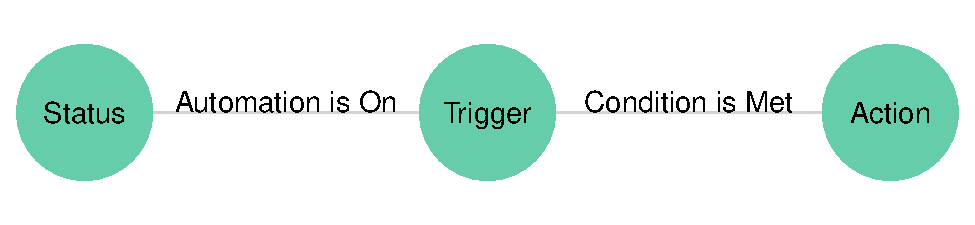
\includegraphics{_main_files/figure-latex/actions diagram-1.pdf}

Automations are commonly used to augment the synced tables feature, send notifications, check data quality, and manipulate or create records.

This automation creates a weekly summary of applicants who applied for a position. Its trigger is time based, then it finds records that match a condition, and finally it generates an email from those records and sends to the appropriate recipients.

\begin{figure}
\centering
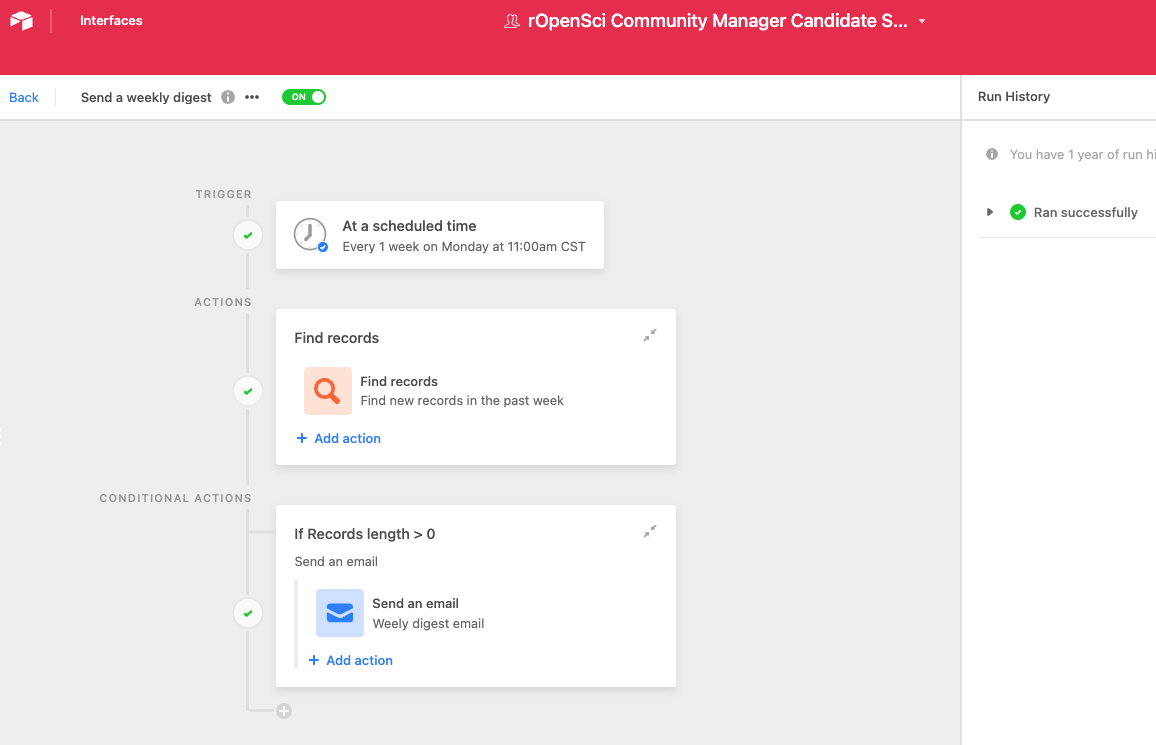
\includegraphics{./images/airtable_Weekly Digest.png}
\caption{airtable weekly summary}
\end{figure}

\hypertarget{scripting-and-blocks-pro-plan-and-above}{%
\subsection{Scripting and Blocks (pro plan and above)}\label{scripting-and-blocks-pro-plan-and-above}}

Scripting uses JavaScript to manipulate a base from within an application in Airtable. Scripting is flexible but has a steep learning curve. The scripting environment Airtable provides can be helpful as it provides code \href{https://en.wikipedia.org/wiki/Lint_(software)}{linting}, direct access to documentation, and example scripts to build from. The major drawback to scripting is that scripts live in the base and files are not version controlled.

\begin{itemize}
\tightlist
\item
  There are a LOT of \href{https://airtable.com/marketplace/category/scripts}{pre-written scripts, in a shared ``marketplace''} to perform automatic actions. Search the marketplace before you start writing bespoke code.
\end{itemize}

Blocks are custom applications built in JavaScript and node.js that add to base functionality. They are created in a development environment outside of Airtable then brought back into platform. There are number of \href{https://www.airtable.com/developers/apps/guides/getting-started}{tutorials for getting started with blocks}.

\hypertarget{using-the-rest-api}{%
\section{Using the REST API}\label{using-the-rest-api}}

All Airtable bases are automatically accessible to authorized users via a REST API. The list of API accessible bases you have access to can be found here: \url{https://airtable.com/api}. By clicking on a base you will be able to see the full API documentation for that base.

\hypertarget{scoped-tokens}{%
\subsection{Scoped Tokens}\label{scoped-tokens}}

Airtable is moving to a \href{https://airtable.com/developers/web/guides/personal-access-tokens}{scoped tokens} based approach to api access. Scoped personal access tokens allow you to create a token for a specific base with specific permissions - e.g.~token has read-only access to a bat sampling base. Using scoped tokens in this way means that if the token is compromised (leaked, stolen, accidentally committed unencrypted to a github repo, etc), you can delete that token to remove any access it might have had and the limited scope means that you know exactly what a person would have been able to access.

To create a personal access token go here: \url{https://airtable.com/create/tokens}

** Remember to save the token in a secure place. Do not store unencrypted tokens on the web (e.g.~pushing them to github).

Airtable has also deployed \href{https://airtable.com/developers/web/api/oauth-reference}{oauth tokens} for all users.

\hypertarget{airtable-and-r}{%
\subsection{Airtable and R}\label{airtable-and-r}}

The Airtable REST API can be used via R with the \href{https://github.com/ecohealthalliance/airtabler}{airtabler package}. EHA has started a fork of the package that has additional functionality so it is recommended to use that version. The original package design works well for exploring the data. Our extension adds additional functionality to help use \texttt{airtabler} in automation via continuous integration such as GitHub Actions.

\begin{verbatim}
devtools::install_github("ecohealthalliance/airtabler")
\end{verbatim}

The Airtable API serves up data as JSON, which has a hierarchical structure similar to a list in R. To handle JSON, \texttt{airtabler} uses the \texttt{jsonlite} package. Its helpful to understand how \texttt{jsonlite} handles different JSON structures when working with more complicated Airtable data. See the \texttt{jsonlite} \href{https://cran.r-project.org/web/packages/jsonlite/vignettes/json-aaquickstart.html}{quick-start guide} for a basic overview. The \href{https://purrr.tidyverse.org/}{\texttt{purr} package} is extremely helpful when dealing with data objects derived from JSON because it facilitates navigating nested data structures.

The \texttt{airtabler} package provides instructions for setting up access to the Airtable API. You will need to follow those instructions for the following examples to work.

\textbf{One to One join}

\begin{verbatim}
library(airtabler)

table1  <-  fetch_all(base = "app49bbyLczZxX9PM",table_name = "One To One")

table2 <- fetch_all(base = "app49bbyLczZxX9PM",table_name = "Table 2")

## Linked records are stored as JSON arrays so they become lists 
## when part of a data frame. Because each array has a length of 1
## we can safely unlist the arrays and add them back as to the 
## data frame.

table1$LinkedRec <- unlist(table1$LinkedRec)

joinedTables <- dplyr::left_join(table1,table2, by = c("LinkedRec"="id"))

recordKey <- joinedTables[c("Name","LinkedRec","Number")]

recordKey

\end{verbatim}

\textbf{One to Many Join}

\begin{verbatim}
library(airtabler)
library(dplyr)
library(purrr)

oneToMany  <-  fetch_all(base = "app49bbyLczZxX9PM",table_name = "One To Many")

table2 <- fetch_all(base = "app49bbyLczZxX9PM",table_name = "Table 2")

# Depending on how you want to work with the data joins are a 
# little trickier here. 

## to replace the values but keep the structure

oneToMany$LinkedRecReplace <- purrr::map(oneToMany$LinkedRec, function(x){
  table2 %>%
    filter(id %in% x) %>%
    select(c("id","Number")) %>% 
    pull("Number")
})

data.frame(
  id = unlist(oneToMany$LinkedRec), 
  label = unlist(oneToMany$LinkedRecReplace)
)
\end{verbatim}

\hypertarget{data-management}{%
\section{Data Management}\label{data-management}}

Because of its flexibility and ease of use, it is extremely important that data
management for airtable be taken seriously. Unlike most other relational databases,
the fundamental properties of your base can be changed easily by multiple users
without warning! Documenting the structure and purpose of your base, as well
as creating regular external backups could save you from catastrophe.

\hypertarget{metadata}{%
\subsection{Metadata}\label{metadata}}

\begin{itemize}
\tightlist
\item
  \textbf{Structural metadata} - Information about a resource that tells you how its
  put together - e.g.~the relationship between a table, field, and automation. With
  the exception of users on the enterprise plan, you must be deliberate about
  creating and maintaining structural metadata for your base.
\end{itemize}

Example of Airtable Structural Metadata:

\begin{itemize}
\tightlist
\item
  \textbf{Descriptive metadata} - Information about a resource that makes it easier to
  find and attribute data. This includes things attributes like author, title, description,
  keywords, etc. This table becomes especially important when data are transitioned
  out of airtable, at the end of a project, or if the base will be shared broadly
  with collaborators.
\end{itemize}

Example of Airtable Descriptive Metadata:

To see the template base, follow this \href{https://airtable.com/invite/l?inviteId=inv5ycCAbIVw1WM3Z\&inviteToken=ef7b72e998a0a69d835244f87f88b6b9b6b1094915239ebc93423e1257fcd72b\&utm_medium=email\&utm_source=product_team\&utm_content=transactional-alerts}{link}

\hypertarget{metadata-for-automations-and-extensions}{%
\subsubsection{Metadata for automations and extensions}\label{metadata-for-automations-and-extensions}}

Automations and extensions live entirely inside airtable. As of August 2022, Airtable introduced a ``Manage Fields'' tab that provides metadata for a specific table, including any automation dependencies. It is not possible to export those dependency tables or the code used in automations automatically. This makes it extremely important to document any automations and extensions outside your base.

\hypertarget{external-backups}{%
\subsection{External Backups}\label{external-backups}}

It is a good idea to create regular external backups of airtable data in the event
that something catastrophic happens to your base or you simply decide you no longer wish
to use airtable as your data store.Unfortunately, airtable does not provide an
off the shelf solution for this. Below are three options for extracting all data
from your base.

\hypertarget{using-airtabler}{%
\subsubsection{Using airtabler}\label{using-airtabler}}

Using \texttt{airtabler::air\_dump()} and \texttt{airtabler::air\_dump\_to\_csv()} functions, you can export all tables to R then create a versioned folder of CSVs. See the \texttt{air\_dump\_to\_csv} help page for more information.

\hypertarget{other-open-source-projects}{%
\subsubsection{Other Open Source Projects}\label{other-open-source-projects}}

UnlyEd - use this template to push airtable backups to AWS S3.

\begin{itemize}
\tightlist
\item
  \url{https://github.com/UnlyEd/airtable-backups-boilerplate}
\end{itemize}

\hypertarget{paid-services}{%
\subsubsection{Paid services}\label{paid-services}}

Sequin - replicate airtable to postGres database
- \url{https://www.sequin.io/sources/airtable}

\hypertarget{r}{%
\section{R}\label{r}}

\href{https://cran.r-project.org}{R} is a free and open-source programming language and software environment for statistical computing and graphics. It was first developed in the early 1990s by Ross Ihaka and Robert Gentleman at the University of Auckland, New Zealand, and is now widely used by statisticians, data analysts, and researchers across various fields.

R provides a wide range of statistical and graphical techniques, including linear and nonlinear modeling, classical statistical tests, time-series analysis, classification, clustering, and more. It also has a large and active community of users and developers who contribute to the development of new packages and extensions for the language.

R is popular in the field of data science, as it provides a powerful and flexible platform for analyzing and visualizing data. It can be used in conjuction with other tools such as Airtable through community-developed packages making it particularly well-suited for the current use-case of the RIG.

\hypertarget{database}{%
\chapter{Database}\label{database}}

The current database is built using \href{https://airtable.com}{Airtable}. The current database has the following schema:

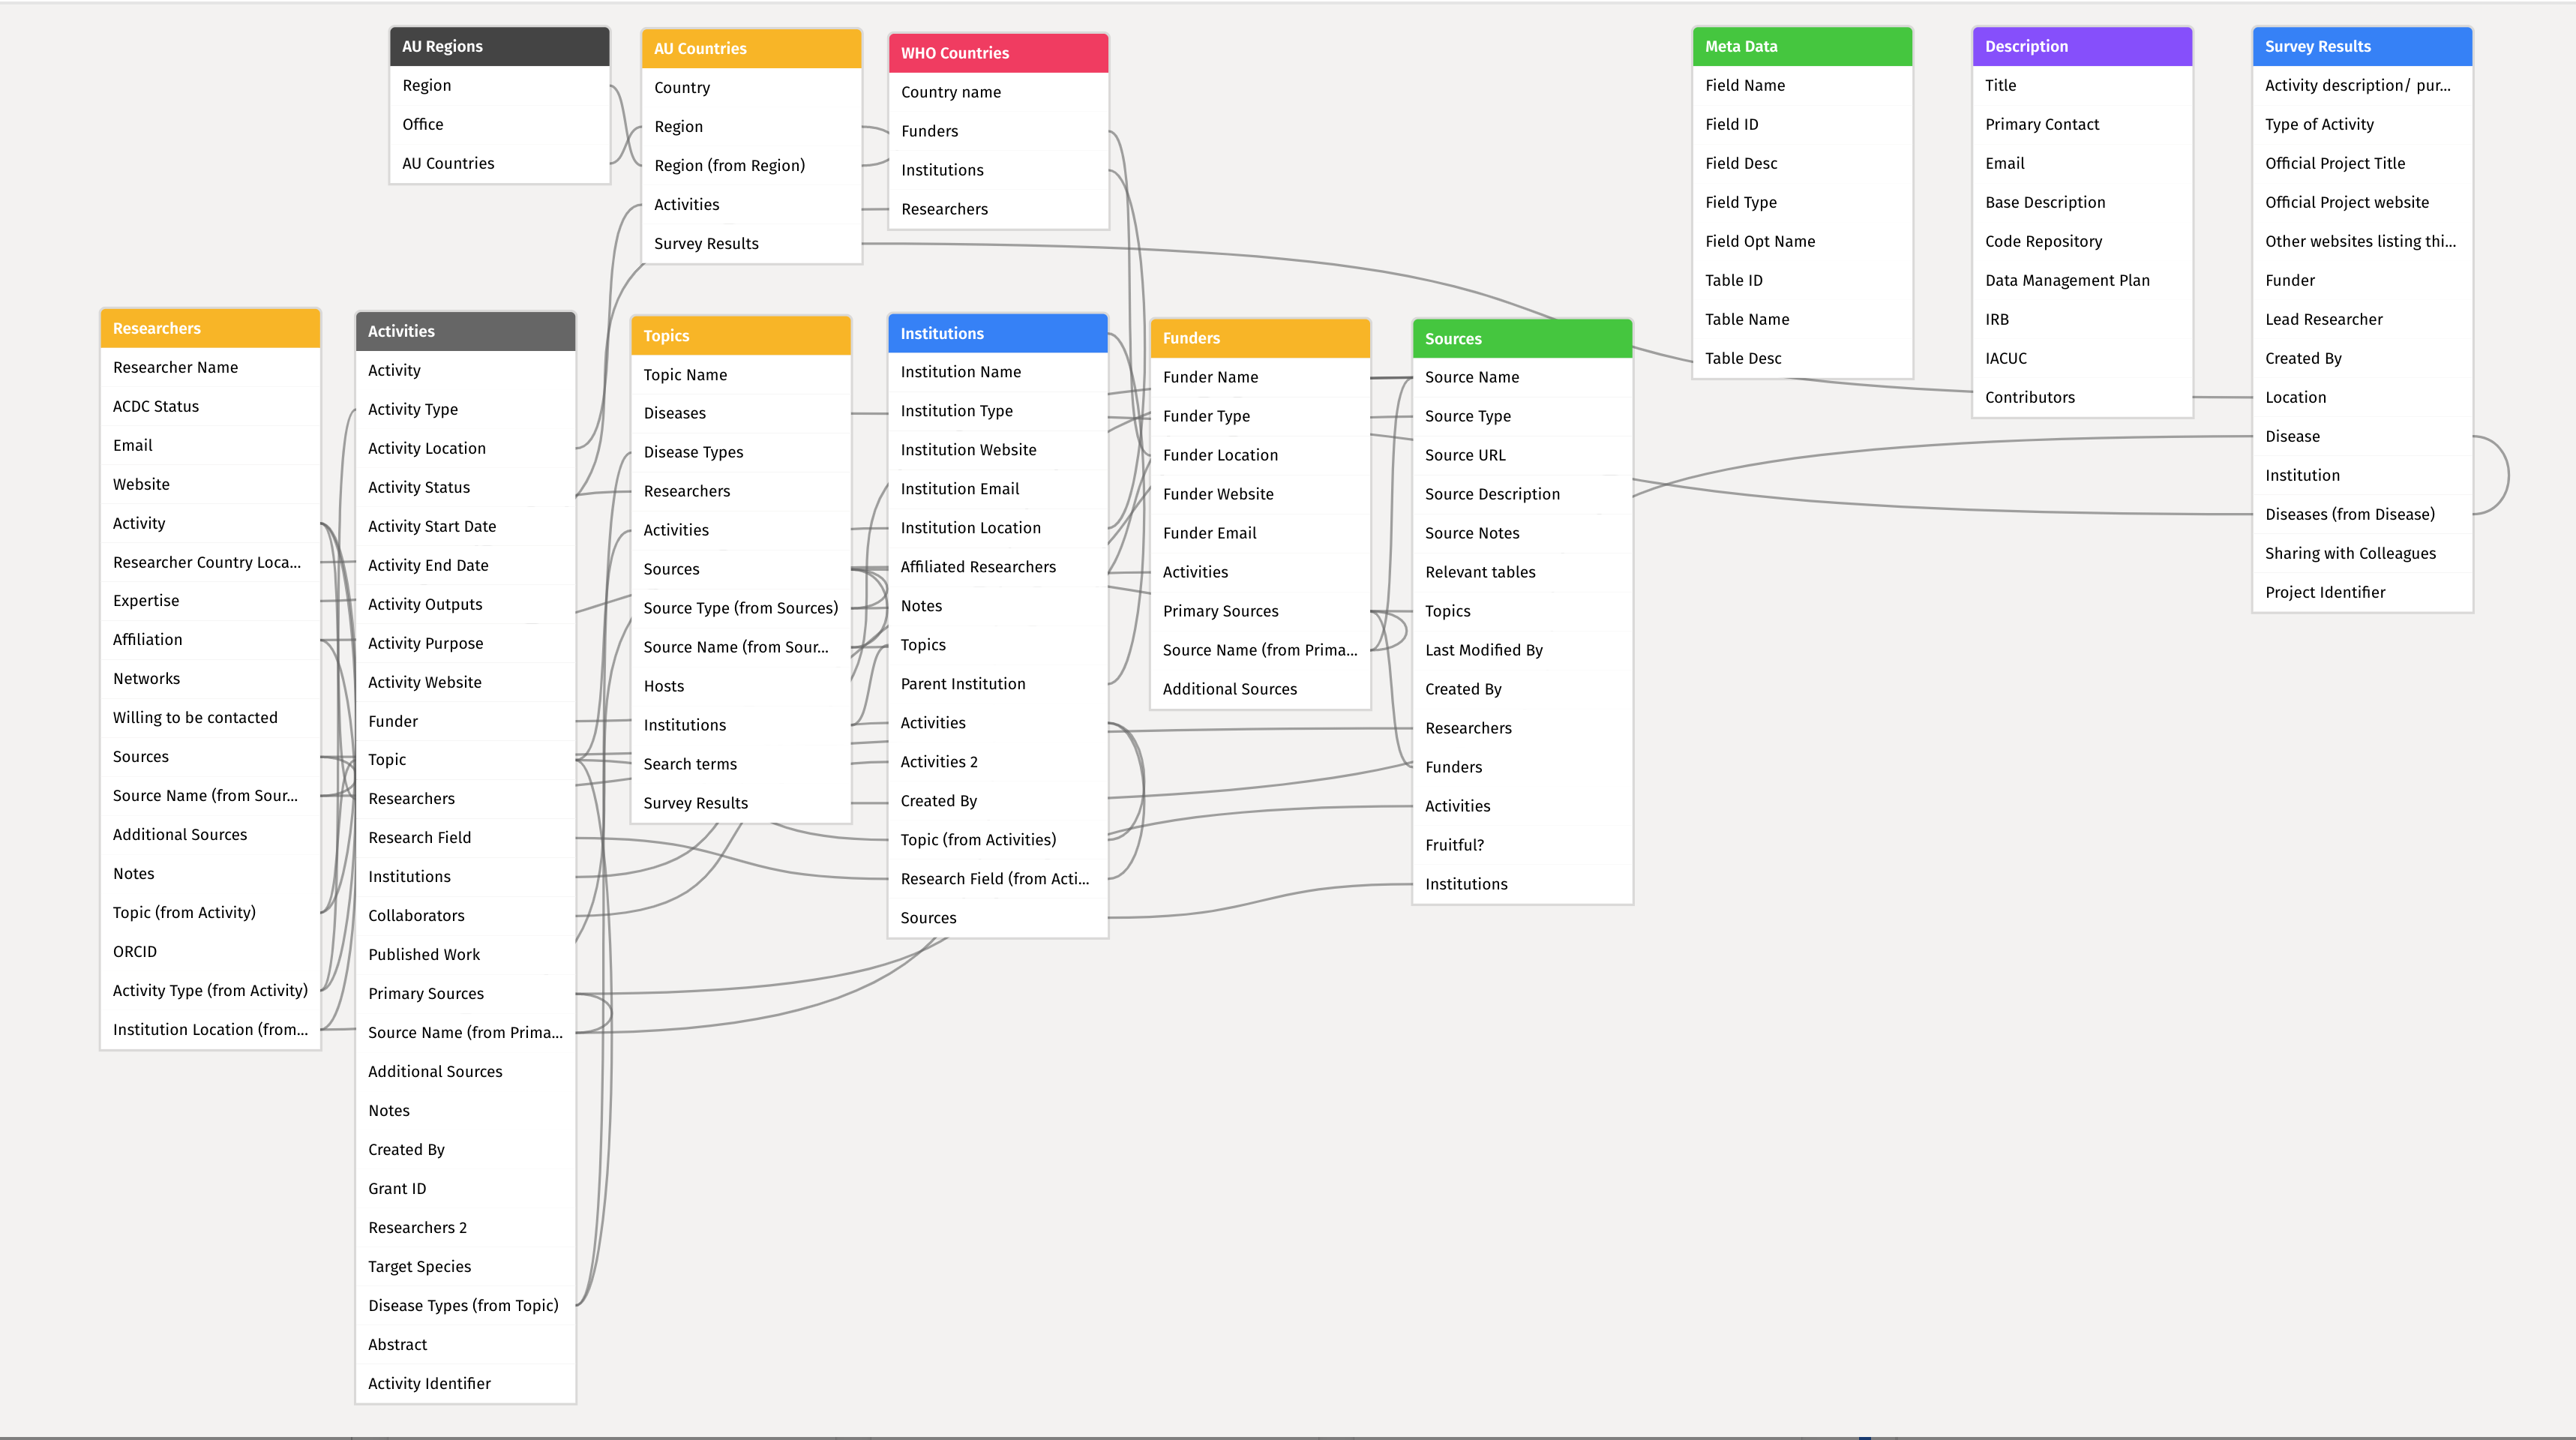
\includegraphics{images/database_schema.png}

This schema can be viewed interactively from here - \url{https://airtable.com/appAL7fJUpBPYtOq4/tblt9ott045tWENcg/viwznxjIFAsTu0jzJ?blocks=bliZ6LV2bkGQNzgKF}

\hypertarget{activities-table}{%
\section{Activities Table}\label{activities-table}}

\hypertarget{table-details}{%
\subsection{Table details}\label{table-details}}

\begin{table}
\centering
\begin{tabular}{l|l|l}
\hline
\textbf{Table ID} & \textbf{Table Name} & \textbf{Table Description}\\
\hline
tbl7emmSomJjnOUQX & Activities & Activities pertain to the formal/official title of the project that has been identified during the database search or survey.\\
\hline
\end{tabular}
\end{table}

\hypertarget{fields-details}{%
\subsection{Fields details}\label{fields-details}}

\begin{table}
\centering
\begin{tabular}{l|l|l|l}
\hline
\textbf{Field Name} & \textbf{Field Description} & \textbf{Field Type} & \textbf{Field Values}\\
\hline
Activity & Activity name & singleLineText & NA\\
\hline
Source Name (from Primary Sources) & Name of primary source & multipleLookupValues & NA\\
\hline
Notes & Internal notes for maintenance & singleLineText & NA\\
\hline
Topic & Activity Topic & multipleRecordLinks & Topics\\
\hline
Grant ID & Grand Identifier & singleLineText & NA\\
\hline
Collaborators & Activity collaborators & multipleRecordLinks & Institutions\\
\hline
Researchers & Researchers involved in activity & multipleRecordLinks & Researchers\\
\hline
Published Work & Links to published work & singleLineText & NA\\
\hline
Activity Outputs & Activity Outputs & multipleSelects & Data, Publication, Report, Guideline/SOP, Archive, Improving Diagnostics, Vaccine development, Therapeutics, Epidemic/Pandemic Preparedness, Biosurveillance technology, Prophylaxis, Surveillance, Improving Vaccine strategies, Training, Risk Assessment, Improving Capacity, Policies\\
\hline
Activity Status & Activity Status & singleSelect & Active, Completed\\
\hline
Activity Website & Activity Website & url & NA\\
\hline
Activity Identifier & Activity identifier & formula & NA\\
\hline
Primary Sources & Primary source of information & multipleRecordLinks & Sources\\
\hline
Additional Sources & Additional sources & singleLineText & NA\\
\hline
Region (from Activity Location) & Region location & multipleLookupValues & NA\\
\hline
Activity Location & Activity location & multipleRecordLinks & AU Countries\\
\hline
Target Species & Target Species & multipleSelects & Humans, Wildlife, Livestock, Vector, Plants, Intermediate Host\\
\hline
Institutions & Institution within which activity is being implemented & multipleRecordLinks & Institutions\\
\hline
Activity End Date & Activity End Date & date & NA\\
\hline
Created By & Person who created the entry & createdBy & NA\\
\hline
Disease Types (from Topic) & Disease types & multipleLookupValues & NA\\
\hline
Activity Start Date & Activity Start Date & date & NA\\
\hline
\end{tabular}
\end{table}

\hypertarget{au-countries-table}{%
\section{AU Countries Table}\label{au-countries-table}}

\hypertarget{table-details-1}{%
\subsection{Table details}\label{table-details-1}}

\begin{table}
\centering
\begin{tabular}{l|l|l}
\hline
\textbf{Table ID} & \textbf{Table Name} & \textbf{Table Description}\\
\hline
tblys7SnjkW4IVY0g & AU Countries & List of Africa Union Countries to select country location information from the topics and activities tables.\\
\hline
\end{tabular}
\end{table}

\hypertarget{fields-details-1}{%
\subsection{Fields details}\label{fields-details-1}}

\begin{table}
\centering
\begin{tabular}{l|l|l|l}
\hline
\textbf{Field Name} & \textbf{Field Description} & \textbf{Field Type} & \textbf{Field Values}\\
\hline
Survey Results & NA & multipleRecordLinks & Survey Results\\
\hline
Country & Full name of country as per WHO/UN nomenclature & singleLineText & NA\\
\hline
Topic (from Activities) & Name of topic identified to the region & multipleLookupValues & NA\\
\hline
Activities & Name of activities identified in the region & multipleRecordLinks & Activities\\
\hline
\end{tabular}
\end{table}

\hypertarget{au-regions-table}{%
\section{AU Regions Table}\label{au-regions-table}}

\hypertarget{table-details-2}{%
\subsection{Table details}\label{table-details-2}}

\begin{table}
\centering
\begin{tabular}{l|l|l}
\hline
\textbf{Table ID} & \textbf{Table Name} & \textbf{Table Description}\\
\hline
tblMEovpjJLMWeCoY & AU Regions & List of Africa Union regions to select appropriate and specific African Union regions information for AU countries, topics, and activities tables.\\
\hline
\end{tabular}
\end{table}

\hypertarget{fields-details-2}{%
\subsection{Fields details}\label{fields-details-2}}

\begin{table}
\centering
\begin{tabular}{l|l|l|l}
\hline
\textbf{Field Name} & \textbf{Field Description} & \textbf{Field Type} & \textbf{Field Values}\\
\hline
AU Countries & Countries within the region based on Africa Union classification & multipleRecordLinks & AU Countries\\
\hline
\end{tabular}
\end{table}

\hypertarget{description-table}{%
\section{Description Table}\label{description-table}}

\hypertarget{table-details-3}{%
\subsection{Table details}\label{table-details-3}}

\begin{table}
\centering
\begin{tabular}{l|l|l}
\hline
\textbf{Table ID} & \textbf{Table Name} & \textbf{Table Description}\\
\hline
tblwapW8nMmUv74GM & Description & The Description table provides overall description of this entire database.\\
\hline
\end{tabular}
\end{table}

\hypertarget{field-details}{%
\subsection{Field details}\label{field-details}}

\begin{table}
\centering
\begin{tabular}{l|l|l|l}
\hline
\textbf{Field Name} & \textbf{Field Description} & \textbf{Field Type} & \textbf{Field Values}\\
\hline
Email & Email for primary contact & email & NA\\
\hline
Primary Contact & Person to correspond with about the base & singleLineText & NA\\
\hline
IRB & Optional: Link to IRB & url & NA\\
\hline
Base Description & Characterization of the base. What is the base describing? & multilineText & NA\\
\hline
Title & Title of the base & singleLineText & NA\\
\hline
Data Management Plan & Link to data management plan & url & NA\\
\hline
Code Repository & Optional: Link to github repo & url & NA\\
\hline
IACUC & Optional: Link to IACUC & singleLineText & NA\\
\hline
\end{tabular}
\end{table}

\hypertarget{funders-table}{%
\section{Funder Table}\label{funders-table}}

\hypertarget{table-details-4}{%
\subsection{Table details}\label{table-details-4}}

\begin{table}
\centering
\begin{tabular}{l|l|l}
\hline
\textbf{Table ID} & \textbf{Table Name} & \textbf{Table Description}\\
\hline
tblDQVkAy8ROTYfFS & Funders & Funders pertain to the entities funding each activity.

The funders' information is retrieved from declared funders for the activities identified during the database search or the survey.\\
\hline
\end{tabular}
\end{table}

\hypertarget{field-details-1}{%
\subsection{Field details}\label{field-details-1}}

\begin{table}
\centering
\begin{tabular}{l|l|l|l}
\hline
\textbf{Field Name} & \textbf{Field Description} & \textbf{Field Type} & \textbf{Field Values}\\
\hline
Funder Type & Type of funder & singleSelect & Charitable organization, Foundation, Pharmaceutical company , Not-for-profit Partnership, NGO, Government Agency, University, Research Institut, Public- public partnership , Public-private partnership\\
\hline
Funder Website & Website of funder & url & NA\\
\hline
Source Name (from Primary Sources) & Source from where funder was identified & multipleLookupValues & NA\\
\hline
Activities & Activities supported by funder & multipleRecordLinks & Activities\\
\hline
Primary Sources & Source from where funder was identified & multipleRecordLinks & Sources\\
\hline
Funder Email & Email of funder & email & NA\\
\hline
\end{tabular}
\end{table}

\hypertarget{institutions-table}{%
\section{Institutions Table}\label{institutions-table}}

\hypertarget{table-details-5}{%
\subsection{Table details}\label{table-details-5}}

\begin{table}
\centering
\begin{tabular}{l|l|l}
\hline
\textbf{Table ID} & \textbf{Table Name} & \textbf{Table Description}\\
\hline
tbldEkEN1kqPi0cx2 & Institutions & Institutions pertain to the entities directly related to or implementing the activity and/or the affiliation of the researcher implementing the activity.\\
\hline
\end{tabular}
\end{table}

\hypertarget{field-details-2}{%
\subsection{Field details}\label{field-details-2}}

\begin{table}
\centering
\begin{tabular}{l|l|l|l}
\hline
\textbf{Field Name} & \textbf{Field Description} & \textbf{Field Type} & \textbf{Field Values}\\
\hline
Institution Email & Email of institution & email & NA\\
\hline
Institution Website & Institution Website & url & NA\\
\hline
Activities & Name of activity identified with institution & multipleRecordLinks & Activities\\
\hline
Sources & Name of primary source & multipleRecordLinks & Sources\\
\hline
Institution Type & Institution Type & singleSelect & Research Institute, University, NGO, National Government Institution, Non-profit Organisation , Hospital, Government Agency, Consortium, Partnership of Institutes, Industry, Charity, Public-private partnetship, International Coalition , Inter-governmental Organisation, Medical Service Provider\\
\hline
Institution Location & Institution location & multipleRecordLinks & WHO Countries\\
\hline
Notes & Internal notes (for maintenance) & singleLineText & NA\\
\hline
Topic (from Activities) & Name of topic identified with the institution & multipleLookupValues & NA\\
\hline
Institution Name & Institution Name & singleLineText & NA\\
\hline
Activities 2 & Additional activities identified with institution & multipleRecordLinks & Activities\\
\hline
\end{tabular}
\end{table}

\hypertarget{researchers-table}{%
\section{Researchers Table}\label{researchers-table}}

\hypertarget{table-details-6}{%
\subsection{Table details}\label{table-details-6}}

\begin{table}
\centering
\begin{tabular}{l|l|l}
\hline
\textbf{Table ID} & \textbf{Table Name} & \textbf{Table Description}\\
\hline
tblt9ott045tWENcg & Researchers & Researchers pertains to the people involved in the activities contained in this database, and maybe involved in a variety of activity types. including but not limited to, research.

Researchers identified during the database search. Information on researchers are primarily retrieved once activities have been identified from the database search process. It is possible that researchers are identified apriori and from which information on topics, funders, sources, institutions, and activities may be identified relevant to the specific researcher. This may happen when the planned/proposed survey is implemented and sent to known researchers who may or may not be in the database to begin with.\\
\hline
\end{tabular}
\end{table}

\hypertarget{field-details-3}{%
\subsection{Field details}\label{field-details-3}}

\begin{table}
\centering
\begin{tabular}{l|l|l|l}
\hline
\textbf{Field Name} & \textbf{Field Description} & \textbf{Field Type} & \textbf{Field Values}\\
\hline
ACDC Status & Is researcher from the Africa CDC? & singleSelect & Non-member, Member\\
\hline
Sources & Name of source & multipleRecordLinks & Sources\\
\hline
Affiliation & Institution researcher is affiliated with. Choices from the institutions table & multipleRecordLinks & Institutions\\
\hline
Topic (from Activity) & Name of topic & multipleLookupValues & NA\\
\hline
Researcher Name & Full name of researcher identified in the search & singleLineText & NA\\
\hline
Notes & Internal notes (for maintenance) & singleLineText & NA\\
\hline
Source Name (from Sources) & Name of source & multipleLookupValues & NA\\
\hline
Additional Sources & Additional sources & singleLineText & NA\\
\hline
Activity Type (from Activity) & Type of activity & multipleLookupValues & NA\\
\hline
Website & Personal website of researcher (if any) & singleLineText & NA\\
\hline
Activity & Activity/activities researchers is involved in & multipleRecordLinks & Activities\\
\hline
Institution Location (from Affiliation) & Name of location where institution is based & multipleLookupValues & NA\\
\hline
Willing to be contacted & Is the researcher willing to be contacted? & checkbox & NA\\
\hline
Expertise & Topic which researcher is considered an expert on. Choices selected from the topics table & multipleRecordLinks & Topics\\
\hline
\end{tabular}
\end{table}

\hypertarget{sources-table}{%
\section{Sources Table}\label{sources-table}}

\hypertarget{table-details-7}{%
\subsection{Table details}\label{table-details-7}}

\begin{table}
\centering
\begin{tabular}{l|l|l}
\hline
\textbf{Table ID} & \textbf{Table Name} & \textbf{Table Description}\\
\hline
tbl71q8ghTcqTybtf & Sources & Sources contain initial set of sources (primarily funders) identified to initiate the database search. These original sources are fully described here - https://ecohealthalliance.github.io/rig-handbook/sources.html. 

From the initial search, other sources were identified from which additional streams of searches were performed.  Currently, the sources table is updated through a primary search of possible sources in addition to the search performed on the original sources list.\\
\hline
\end{tabular}
\end{table}

\hypertarget{field-details-4}{%
\subsection{Field details}\label{field-details-4}}

\begin{table}
\centering
\begin{tabular}{l|l|l|l}
\hline
\textbf{Field Name} & \textbf{Field Description} & \textbf{Field Type} & \textbf{Field Values}\\
\hline
Source Type & Type of primary source & singleSelect & Website text page, Website table, Website search, Downloadable document in PDF, Downloadable document in XLSX, Downloadable document in CSV, Downloadable document in DOCX, A form of database, Website text page, Website search, Links to downloadable documents in PDF, Website table, Website search\\
\hline
Source Notes & Internal notes for primary source (for maintenance) & multilineText & NA\\
\hline
Topics & Topics identified from primary source & multipleRecordLinks & Topics\\
\hline
Relevant tables & Notes on relevant tables found from primary source & multipleSelects & Researchers, Topics, Activities, Funders, Institutions, Countries\\
\hline
Funders & Funders identified from primary source & multipleRecordLinks & Funders\\
\hline
Source Name & Name of primary source & singleLineText & NA\\
\hline
Created By & Person who created the entry & createdBy & NA\\
\hline
Researchers & Name of researcher identified from primary source & multipleRecordLinks & Researchers\\
\hline
Institutions & Institution identified from primary source & multipleRecordLinks & Institutions\\
\hline
Fruitful? & Was source relevant/contributory? & singleSelect & Yes, No, Partially, Not reviewed yet\\
\hline
\end{tabular}
\end{table}

\hypertarget{survey-results-table}{%
\section{Survey Results Table}\label{survey-results-table}}

\hypertarget{table-details-8}{%
\subsection{Table details}\label{table-details-8}}

\begin{table}
\centering
\begin{tabular}{l|l|l}
\hline
\textbf{Table ID} & \textbf{Table Name} & \textbf{Table Description}\\


\hline
\end{tabular}
\end{table}

\hypertarget{field-details-5}{%
\subsection{Field details}\label{field-details-5}}

\begin{table}
\centering
\begin{tabular}{l|l|l|l}
\hline
\textbf{Field Name} & \textbf{Field Description} & \textbf{Field Type} & \textbf{Field Values}\\
\hline
Activity description/ purpose & Description of activity & multilineText & NA\\
\hline
Sharing with Colleagues & Is respondent going to share with colleagues? & singleLineText & NA\\
\hline
Lead Researcher & Name of lead researcher & singleLineText & NA\\
\hline
Created By & Name of survey respondent & createdBy & NA\\
\hline
Other websites listing this project & Other website listings for this project & singleLineText & NA\\
\hline
Funder & Name of funder for this project & singleLineText & NA\\
\hline
Official Project Title & Official project title & singleLineText & NA\\
\hline
Official Project website & Official project website & singleLineText & NA\\
\hline
Type of Activity & Activity type & multipleSelects & Surveillance, Clinical Trial, Basic Science, Behavioural Science, Epidemiology , Other\\
\hline
Disease & Name of disease relevant to activity/project & multipleRecordLinks & Topics\\
\hline
\end{tabular}
\end{table}

\hypertarget{topics-table}{%
\section{Topics Table}\label{topics-table}}

\hypertarget{table-details-9}{%
\subsection{Table details}\label{table-details-9}}

\begin{table}
\centering
\begin{tabular}{l|l|l}
\hline
\textbf{Table ID} & \textbf{Table Name} & \textbf{Table Description}\\
\hline
tblIyWqnGcVE4mGRg & Topics & Topics pertain to the disease names and disease types. 

The topics table contains disease types/disease entities of interest to the Africa CDC based on their priorities (as described in their Framework document) and is continually updated with whatever disease/disease entity/disease type were deemed relevant by the database contributor.\\
\hline
\end{tabular}
\end{table}

\hypertarget{field-details-6}{%
\subsection{Field details}\label{field-details-6}}

\begin{table}
\centering
\begin{tabular}{l|l|l|l}
\hline
\textbf{Field Name} & \textbf{Field Description} & \textbf{Field Type} & \textbf{Field Values}\\
\hline
Sources & Name of Source & multipleRecordLinks & Sources\\
\hline
Diseases & Disease entity related/relevant to the field/topic of interest & multipleSelects & HIV, TB, COVID-19, Monkeypox, Lassa fever, Bat flu, Avian flu, Swine flu, Ebola virus disease, Marburg virus disease, Marburg haemorrhagic fever, H7N9, H5N1, H1N1, H1N2, H3N2, Plague, Anthrax, Crimean-Congo Haemorrhagic Fever, Rift Valley Fever, Nipah Virus, Brucellosis, undulant fever, Malta fever, Mediterranean fever, Hantavirus haemorrhagic fever with renal syndrome, Hantavirus pulmonary syndrome, Q fever, Chikungunya, Henipavirus, Ghanaian bat henipavirus, Leptospirosis, Weill's disease, West Nile Fever, Zika fever, Dengue fever, African trypanosomiasis, Chagas disease, Yellow fever, Malaria, Re-emerging viruses, Visceral Leishmaniasis, Kala-azar, Cutaneous leishmaniasis , Hepatitis E , Viral Hepatitis, Hepatitis C, Hepatitis B, Leprosy, Hookworm, Schistosomiasis, Ascariasis, Trichuriasis, Lymphatic filariasis, Trachoma, Buruli ulcer, Dracunculiasis, Bilharzia, Whipworm Infection, Elephantiasis, Guinea-worm disease , Burkitt lymphoma, Cryptococcal meningitis, Kaposi sarcoma, schistosomiasis, Viral haemorrhagic fever, Rabies\\
\hline
Activity Location (from Activities) & Name of location of activity in which topic was identified & multipleLookupValues & NA\\
\hline
Survey Results & Results from survey & multipleRecordLinks & Survey Results\\
\hline
Search terms & Search terms used to identify topic & multipleSelects & antimycobacterial, anti-mycobacterial, COVID-19, coronavirus, omicron, rifampicin, ritonavir, darunavir, dolutegravir, MIS-C, HVTN, ART, antiretroviral, lopinavir, bedaquiline, clofazimine, isoniazid, pyrazinamide, antitubercular, tenofovir disoproxil fumarate, emtricitabine, dolutegravir , efavirenz, tubercular, drug-resistant, AMR, raltegravir, DR-, DR-TB, helminth, TBM, fluke, wildlife sampling, biosurveillance, surveillance network, seroprevalence, detection of \_\_, monitoring of \_\_, seroevidence, identification of \_\_, seropositive, seroepidemiological, survey, screened, \_\_ prevalence\\
\hline
Disease Types & Type/category to which disease is grouped under & multipleSelects & infectious disease, viral, bacterial, parasitic, vector-bourne, zoonotic, virus, soil-transmitted\\
\hline
Institutions & Institutions & multipleRecordLinks & Institutions\\
\hline
Region (from Activity Location) (from Activities) & Name of region where topic was identified & multipleLookupValues & NA\\
\hline
Source Name (from Sources) & Name of source & multipleLookupValues & NA\\
\hline
Topic Name & Field or topic of interest relevant to infectious disease and other relevant fields & singleLineText & NA\\
\hline
Activities & Name of activity in which topic was identified & multipleRecordLinks & Activities\\
\hline
Researchers & Name of researcher identified with the topic & multipleRecordLinks & Researchers\\
\hline
\end{tabular}
\end{table}

\hypertarget{who-countries-table}{%
\section{WHO Countries Table}\label{who-countries-table}}

\hypertarget{table-details-10}{%
\subsection{Table details}\label{table-details-10}}

\begin{table}
\centering
\begin{tabular}{l|l|l}
\hline
\textbf{Table ID} & \textbf{Table Name} & \textbf{Table Description}\\
\hline
tblWRh0rWAuXODyb7 & WHO Countries & List of WHO countries used to indicate the location information for the researchers, funders, and institutions tables\\
\hline
\end{tabular}
\end{table}

\hypertarget{field-details-7}{%
\subsection{Field details}\label{field-details-7}}

\begin{table}
\centering
\begin{tabular}{l|l|l|l}
\hline
\textbf{Field Name} & \textbf{Field Description} & \textbf{Field Type} & \textbf{Field Values}\\
\hline
Funders & Name of funder identified in the specific country & multipleRecordLinks & Funders\\
\hline
Institutions & Name of institution identified in the specific country & multipleRecordLinks & Institutions\\
\hline
Country name & Short name of country as per WHO listing & singleLineText & NA\\
\hline
\end{tabular}
\end{table}

\hypertarget{sources}{%
\chapter{Sources}\label{sources}}

Following is an initial list of sources of information used for the RIG database.

The initial search performed was non-systematic and focused primarily on a known funder of global research related/relevant to the topics of interest for the database . The main aim of focusing first on this limited and focused search was to get a sense of what information is available from such bodies/organisations, and the limitations of the information available. This is based on an initial idea that research funders would tend to have a system of collecting/archiving information on research they have funded. The expectation was that at the minimum, the information available from funders would lead to identifying further sources of information relevant to the ACDC database specifically those of research groups/institutions particularly those based in countries/regions within Africa. This initial search will hopefully inform a more systematic and informed search strategy for the database information.

\hypertarget{ukri}{%
\section{UKRI}\label{ukri}}

\href{https://www.ukri.org/}{UK Research and Innovation or UKRI} is a non-departmental public body in the United Kingdom that was established in 2018. It brings together the seven UK Research Councils, \href{https://www.ukri.org/councils/innovate-uk/}{Innovate UK}, and \href{https://www.ukri.org/councils/research-england/}{Research England}, which were previously separate organizations, to create a single body that oversees research and innovation funding and strategy in the UK.

The seven UK Research Councils are:

\begin{enumerate}
\def\labelenumi{\arabic{enumi}.}
\tightlist
\item
  Arts and Humanities Research Council (AHRC)
\item
  Biotechnology and Biological Sciences Research Council (BBSRC)
\item
  Engineering and Physical Sciences Research Council (EPSRC)
\item
  Economic and Social Research Council (ESRC)
\item
  Medical Research Council (MRC)
\item
  Natural Environment Research Council (NERC)
\item
  Science and Technology Facilities Council (STFC)
\end{enumerate}

Innovate UK is the UK's innovation agency, which provides funding and support for innovative businesses and projects.

Research England is responsible for funding and overseeing research in English universities and higher education institutions.

UKRI's main role is to drive innovation and research in the UK and to support research and development that benefits society and the economy. It funds research projects, provides support to researchers, promotes international collaboration, and works to ensure that research and innovation are integrated with government policies and priorities.

Of these various groups within UKRI, we further focused on the \href{https://www.ukri.org/councils/bbsrc/}{Biotechnology and Biological Sciences Research Council (BBSRC)}, \href{https://www.ukri.org/councils/mrc/}{Medical Research Council (MRC)}, \href{https://www.ukri.org/councils/stfc/}{Science and Technology Facilities Council (STFC)}, \href{https://www.ukri.org/councils/innovate-uk/}{Innovate UK}, and \href{https://www.ukri.org/councils/research-england/}{Research England}.

\hypertarget{wellcome}{%
\section{Wellcome Trust}\label{wellcome}}

The Wellcome Trust is a global charitable foundation based in the UK. It was established in 1936 by Sir Henry Wellcome, a pharmaceutical entrepreneur and philanthropist. The Wellcome Trust is one of the largest charitable organizations in the world, with an endowment of over £29 billion.

The Trust's mission is to improve health by supporting scientists, researchers, and innovators in their work to understand, treat, and prevent disease. The Trust funds research in areas such as neuroscience, genetics, infectious diseases, and global health. It also provides support for public engagement with science, education and training for scientists, and the translation of research into practical applications that benefit patients and communities.

The Wellcome Trust is known for its long-term, strategic approach to funding research, and for its commitment to open science and data sharing. It also operates the Wellcome Collection, a public venue in London that hosts exhibitions and events related to health, medicine, and science.

\hypertarget{nih}{%
\section{National Insitutes of Health}\label{nih}}

The National Institutes of Health (NIH) is a biomedical research agency of the United States federal government. It is the largest biomedical research institution in the world, with its main campus located in Bethesda, Maryland. The NIH is composed of 27 separate institutes and centers, each with a specific research focus, and is responsible for conducting and funding research in a wide range of areas, including cancer, genetics, infectious diseases, and neuroscience.

The NIH was founded in 1887 as the Hygienic Laboratory and was later renamed the National Institutes of Health in 1930. Today, it is one of the world's foremost centers for medical research, with a mission to seek fundamental knowledge about the nature and behavior of living systems and to apply that knowledge to enhance health, lengthen life, and reduce illness and disability. The NIH is funded by the U.S. government through the Department of Health and Human Services and operates under the direction of the Office of the Director.

\hypertarget{nsf}{%
\section{National Science Foundation}\label{nsf}}

The National Science Foundation (NSF) is an independent federal agency of the United States government that supports fundamental research and education across all fields of science and engineering. The NSF was established by the National Science Foundation Act of 1950 and has a budget of around \$8 billion.

The NSF funds research and education in areas such as mathematics, computer science, physics, chemistry, biology, social sciences, and engineering. It supports individual researchers, small teams, and large interdisciplinary research collaborations through a competitive, merit-based process of proposal submission and review. The NSF also supports the development of science, technology, engineering, and mathematics (STEM) education at all levels, from K-12 through graduate education.

The NSF operates through several directorates and offices, each with a specific research focus or mission, such as the Directorate for Biological Sciences, the Directorate for Social, Behavioral and Economic Sciences, and the Office of Polar Programs. The NSF works to advance scientific discovery, promote science education and outreach, and promote innovation and economic growth through its investments in research and education.

\hypertarget{darpa}{%
\section{Defense Advanced Research Projects Agency}\label{darpa}}

The Defense Advanced Research Projects Agency is a research and development agency of the United States Department of Defense that is responsible for the development of emerging technologies for use by the military.

DARPA was established in 1958 in response to the Soviet Union's launch of Sputnik, the first artificial satellite, and has been involved in a number of high-profile technological innovations, including the development of the Internet, GPS, and stealth technology.

DARPA's mission is to maintain the technological superiority of the U.S. military by sponsoring and conducting research in a wide range of fields, including artificial intelligence, robotics, biotechnology, materials science, and aerospace technology. DARPA works with academic researchers, private companies, and other government agencies to develop and test new technologies, and it is known for its high-risk, high-reward approach to research and development.

Some of DARPA's current research initiatives include the development of hypersonic weapons, the creation of autonomous drone swarms, and the development of brain-machine interfaces for use in treating neurological disorders. DARPA's work has had significant impacts on both military and civilian technology, and the agency is seen as a leader in cutting-edge research and development.

\hypertarget{clinicaltrials.gov}{%
\section{ClinicalTrials.gov}\label{clinicaltrials.gov}}

ClinicalTrials.gov is a publicly accessible database of clinical trials that are being conducted worldwide. It is maintained by the National Library of Medicine, a part of the National Institutes of Health (NIH) in the United States.

The database provides information on clinical trials for a wide range of diseases and conditions, including both interventional and observational studies. It includes information about the purpose of the trial, who may participate, where the trial is being conducted, and the status of the trial, such as whether it is recruiting participants or has been completed.

ClinicalTrials.gov was created in response to a 1997 law requiring the registration of clinical trials for certain serious or life-threatening diseases or conditions. Since then, the database has grown to include information on thousands of trials from around the world.

ClinicalTrials.gov is an important resource for researchers, healthcare professionals, and members of the public who are interested in clinical research. It can be used to identify ongoing or completed trials, learn about the purpose and design of a study, and find out how to participate in a trial. It also serves as a platform for researchers to share their results and comply with the requirements of various funding agencies and regulatory bodies.

\hypertarget{gepris}{%
\section{GEPRIS}\label{gepris}}

Geförderte Projekte in der Forschung und Entwicklung (Funded Projects in Research and Development) or GEPRIS is an online database of research projects funded by the German Research Foundation (DFG).

The DFG is the largest independent research funding organization in Germany and funds projects across all scientific disciplines, from the humanities and social sciences to the natural and life sciences. GEPRIS provides information about the projects that the DFG has funded, including their aims, methods, and outcomes, as well as the institutions and researchers involved.

Researchers and members of the public can use GEPRIS to search for projects that have been funded by the DFG, and to access information about these projects. The database includes information about ongoing and completed projects, and users can search by various criteria, such as by researcher name, institution, scientific discipline, or project title.

GEPRIS is a valuable tool for researchers to identify potential collaborators, explore research trends, and find information about the funding landscape in their field. It is also useful for members of the public who are interested in learning about the research being conducted in Germany and the impact of this research on society.

\hypertarget{edctp}{%
\section{EDCTP}\label{edctp}}

European and Developing Countries Clinical Trials Partnership or EDCTP is a public-public partnership between countries in Europe and sub-Saharan Africa, established in 2003, with the aim of accelerating the development of new clinical interventions to fight infectious diseases that disproportionately affect Africa.

The partnership's mission is to improve the health of people in Africa by supporting the development of new medicines, vaccines, and other health interventions to prevent and treat diseases such as HIV/AIDS, tuberculosis, malaria, and neglected infectious diseases. EDCTP supports collaborative research projects that bring together scientists, institutions, and countries from both regions to conduct clinical trials and other research activities.

EDCTP works with a range of partners, including national governments, research institutions, civil society organizations, and the private sector, to support research that is relevant and responsive to the needs of African communities. It also provides training and capacity-building opportunities to support the development of sustainable health research infrastructure and expertise in Africa.

The partnership is funded by the European Union, its member states, and other donors. Since its inception, EDCTP has supported over 100 collaborative research projects and played a key role in advancing the development of new interventions for infectious diseases that affect the people of Africa.

\hypertarget{glopidr}{%
\section{GLOPID-R}\label{glopidr}}

Global Research Collaboration for Infectious Disease Preparedness or GLOPID-R is an international partnership that aims to strengthen global research efforts in the field of infectious disease preparedness. The partnership was established in response to the 2014 Ebola outbreak in West Africa, which highlighted the need for improved global coordination and collaboration in research and development for emerging and re-emerging infectious diseases.

GLOPID-R brings together stakeholders from the global health community, including research funders, policy-makers, researchers, and public health organizations. The partnership aims to promote international cooperation and coordination in research to accelerate the development of new tools and approaches to prevent, detect, and respond to infectious disease outbreaks.

GLOPID-R's main objectives include identifying research priorities for infectious disease preparedness, coordinating research efforts across different regions and countries, and promoting capacity building and knowledge exchange to strengthen global health research infrastructure.

The partnership focuses on a range of infectious diseases, including those caused by emerging and re-emerging pathogens, neglected tropical diseases, and antimicrobial resistance. It works to support research efforts across the entire spectrum of infectious disease preparedness, from basic research to clinical trials and implementation research.

GLOPID-R is supported by a range of funding agencies and partners from around the world and is seen as an important platform for promoting global cooperation and collaboration in infectious disease research and preparedness.

\hypertarget{nrfza}{%
\section{NRF South Africa}\label{nrfza}}

The National Research Foundation of South Africa (NRF) is an independent organization that promotes and supports research and innovation in all fields of science, engineering, technology, and social sciences in South Africa. The NRF was established in 1999 through the National Research Foundation Act and operates under the jurisdiction of the Department of Science and Innovation.

The NRF provides funding, develops policies, and manages research infrastructure to support South African researchers and institutions. It also fosters international collaboration in research, and supports the training and development of the next generation of researchers through various funding and fellowship schemes.

The NRF provides funding through a number of programs, including competitive grants, fellowships, and research chairs. It also supports the development of research infrastructure and the establishment of research centers of excellence.

In addition to providing funding and support for research, the NRF plays a key role in developing research policies and strategies at the national level. It advises the South African government on research priorities and is involved in various initiatives aimed at promoting science, technology, and innovation in the country.

The NRF is an important organization for the South African research community and has been instrumental in advancing the country's research and innovation capabilities. Its funding and support have contributed to numerous scientific discoveries and innovations in a wide range of fields, including health, energy, and the environment.

\hypertarget{updates}{%
\chapter{Updates}\label{updates}}

The current update process of the RIG database is summarised in this workflow:

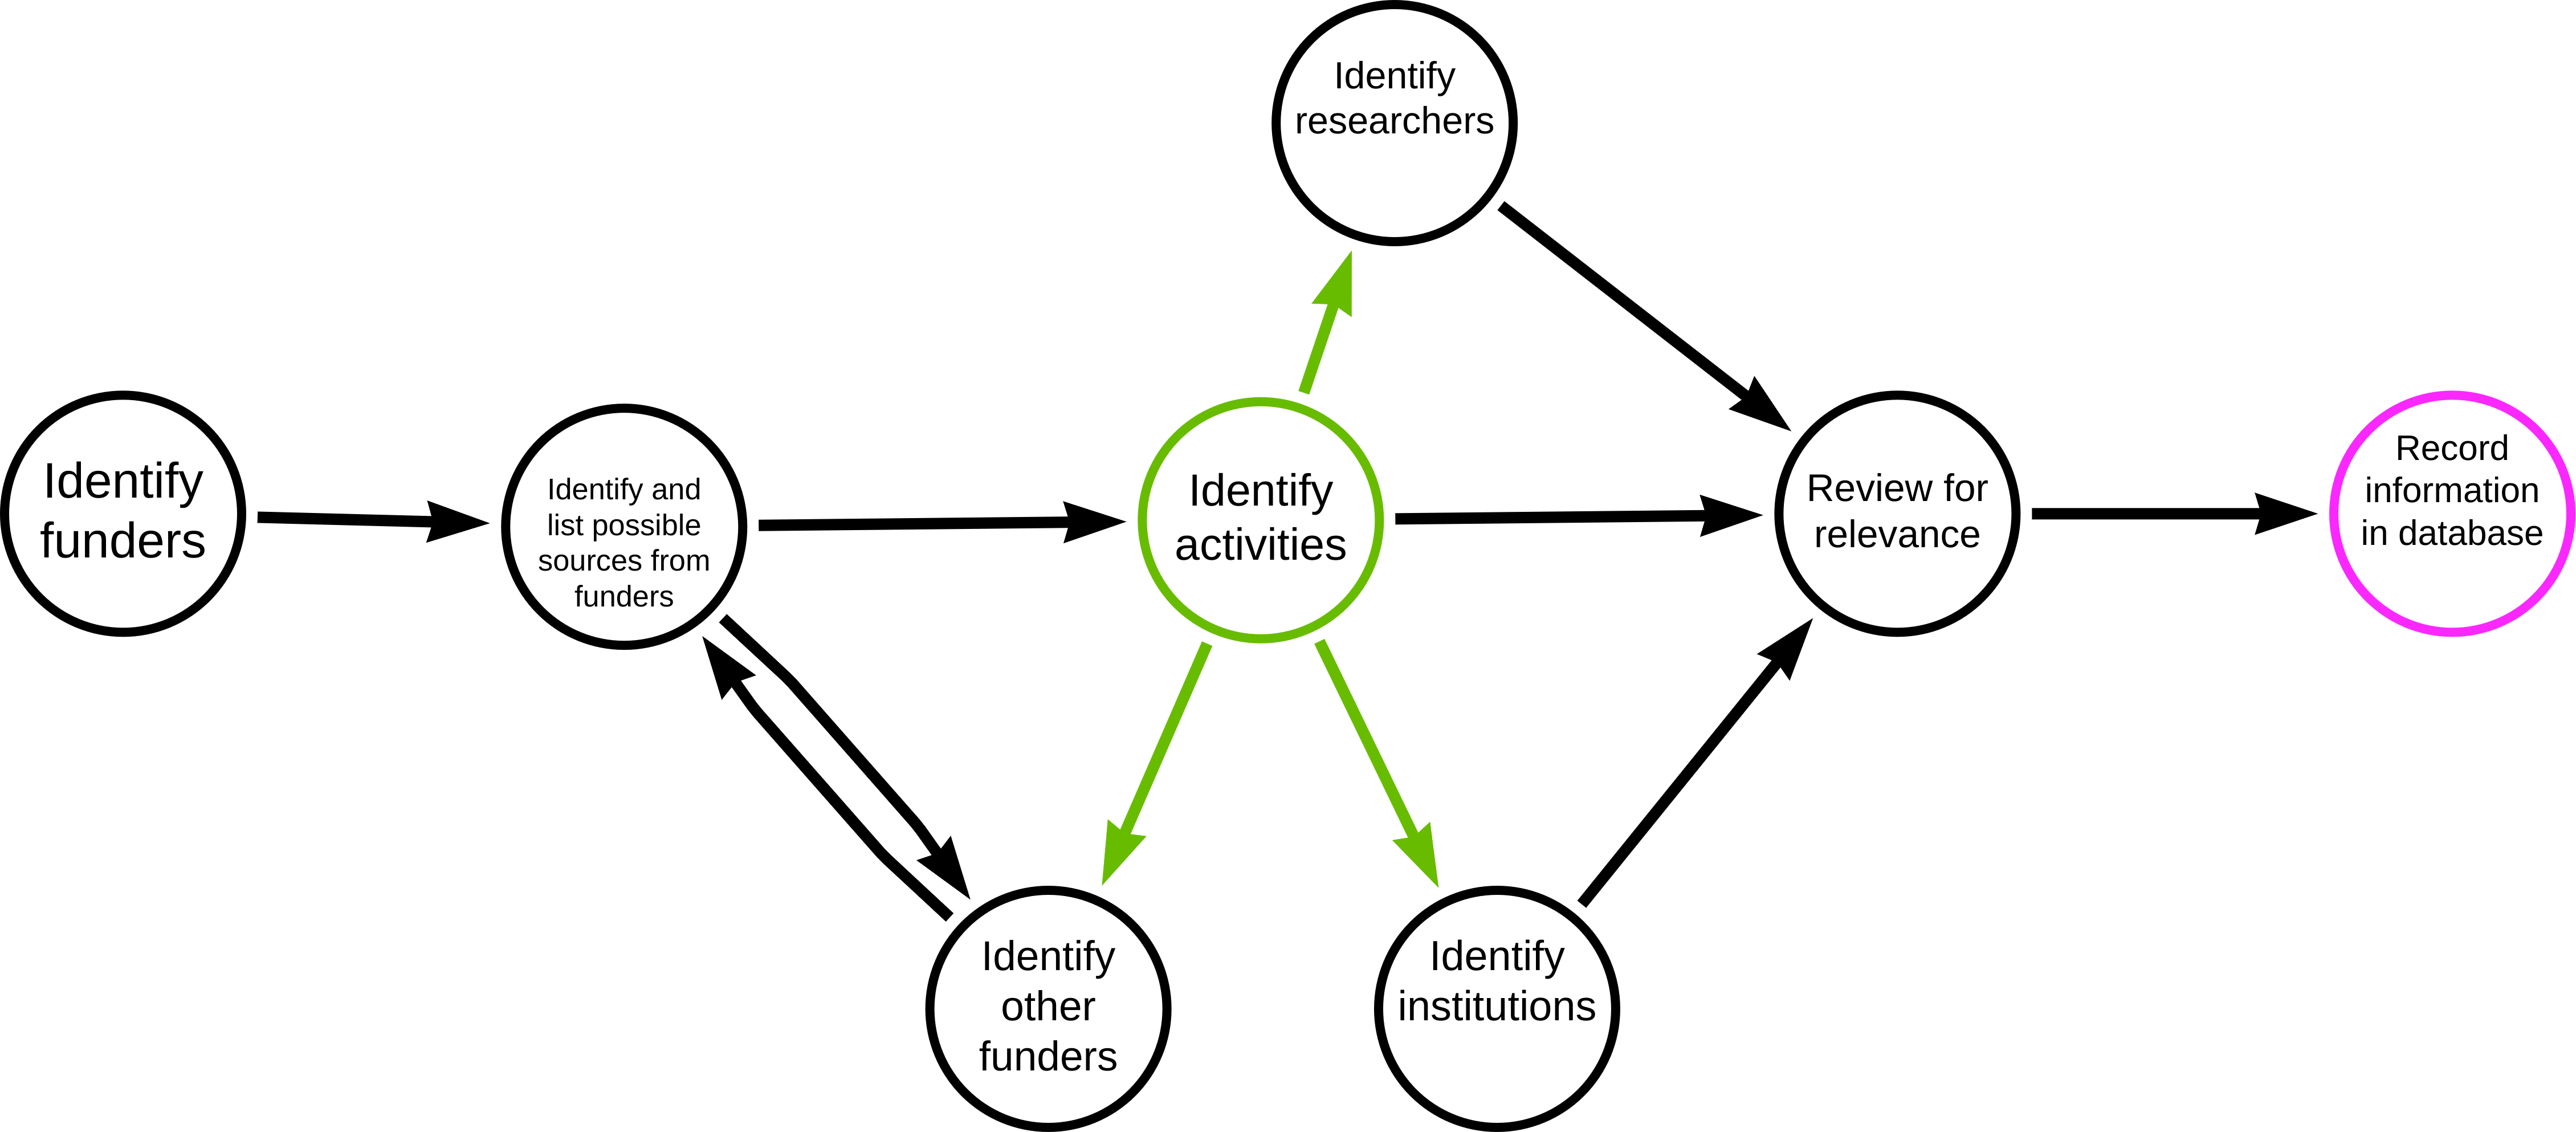
\includegraphics{images/initial-acdc-db-search_NK.png}

Following are the source-specific process of updating or retrieving information for the RIG database.

\hypertarget{update-wellcome}{%
\section{Wellcome Trust Grant Funding Data}\label{update-wellcome}}

\hypertarget{general-information}{%
\subsection{General Information}\label{general-information}}

Using the downloadable spreadsheet of funds awarded between 01st of October 2005 and 4th of May 2022 found at \url{https://cms.wellcome.org/sites/default/files/2022-05/Wellcome-grants-awarded-1-October-2005-to-04-05-2022.xlsx}, the following steps were taken to retrieve relevant information for the database:

\hypertarget{how-to-update}{%
\subsection{How to update}\label{how-to-update}}

Please note that the steps below were done using the current available spreadsheet from the Wellcome Trust website and added the relevant projects to the RIG database. These steps can therefore be used as a guide for how to update the database with new information in the future to when the Wellcome Trust publishes its most up-to-date spreadsheet.

\begin{enumerate}
\def\labelenumi{\arabic{enumi}.}
\item
  Go to column J -- Recipient Org:Country -\textgreater{} deselect all and then select all the African countries in the list
\item
  Go to column N -- Planned end date -\textgreater{} select all the years in the future
\item
  These two steps reduced the list from 19,833 projects to 111 projects
\item
  Read the project title and decide if the project is relevant for our database or not
\item
  If unsure, read the abstract -- that also helps to identify the keywords to tag the project within our database
\item
  If the project is relevant transfer all the information into our database
\end{enumerate}

\textbf{Note:} This method is only able to detect projects/activities where an African organisation itself holds the grant. It does not detect projects where African researchers are involved as collaborators. The spreadsheet does not list collaborators on projects, so it's yet to be determined how we will identify projects on which African research institutes collaborate with international organisations being awarded the grant.

\hypertarget{update-clinicaltrials}{%
\section{ClinicalTrials.gov}\label{update-clinicaltrials}}

\hypertarget{how-to-update-1}{%
\subsection{How to update}\label{how-to-update-1}}

Following are steps taken to extract data from \href{https://clinicaltrials.gov/}{ClinicalTrials.gov}.

\begin{enumerate}
\def\labelenumi{\arabic{enumi}.}
\tightlist
\item
  Start with searching a disease/topic of interest
\end{enumerate}

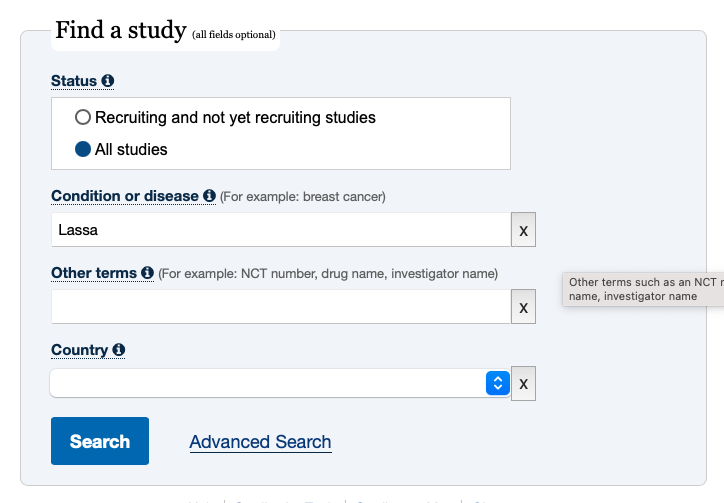
\includegraphics{images/clinicaltrial1.png}

\begin{enumerate}
\def\labelenumi{\arabic{enumi}.}
\setcounter{enumi}{1}
\tightlist
\item
  On the results page apply the following filters to look for active studies
\end{enumerate}

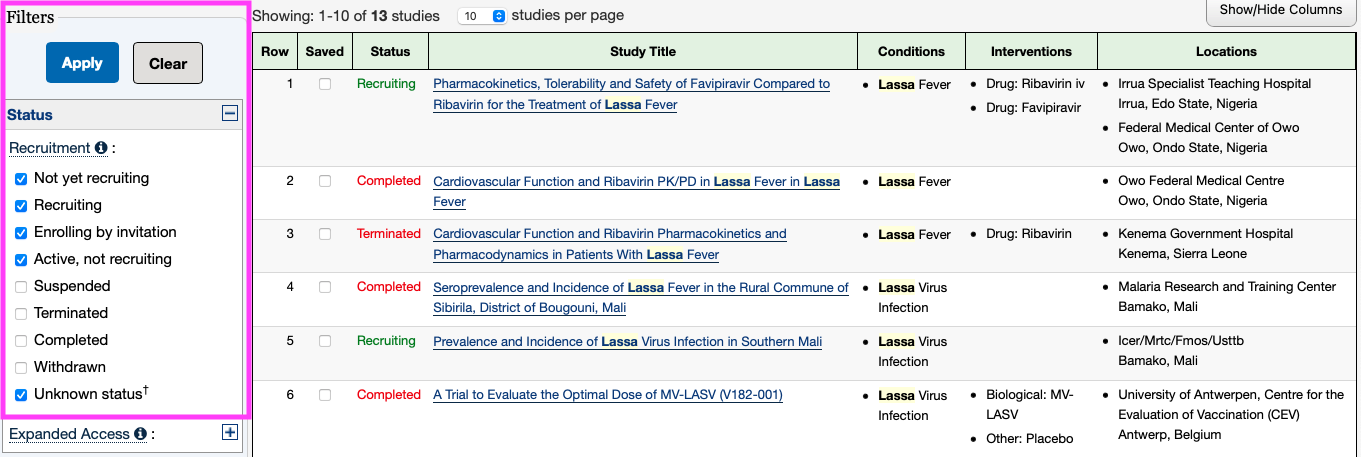
\includegraphics{images/clinicaltrial2.png}

\begin{enumerate}
\def\labelenumi{\arabic{enumi}.}
\setcounter{enumi}{2}
\tightlist
\item
  Click on `Apply' and then look manually through the column `Locations' of the list of the results to find studies that take place in African countries
\end{enumerate}

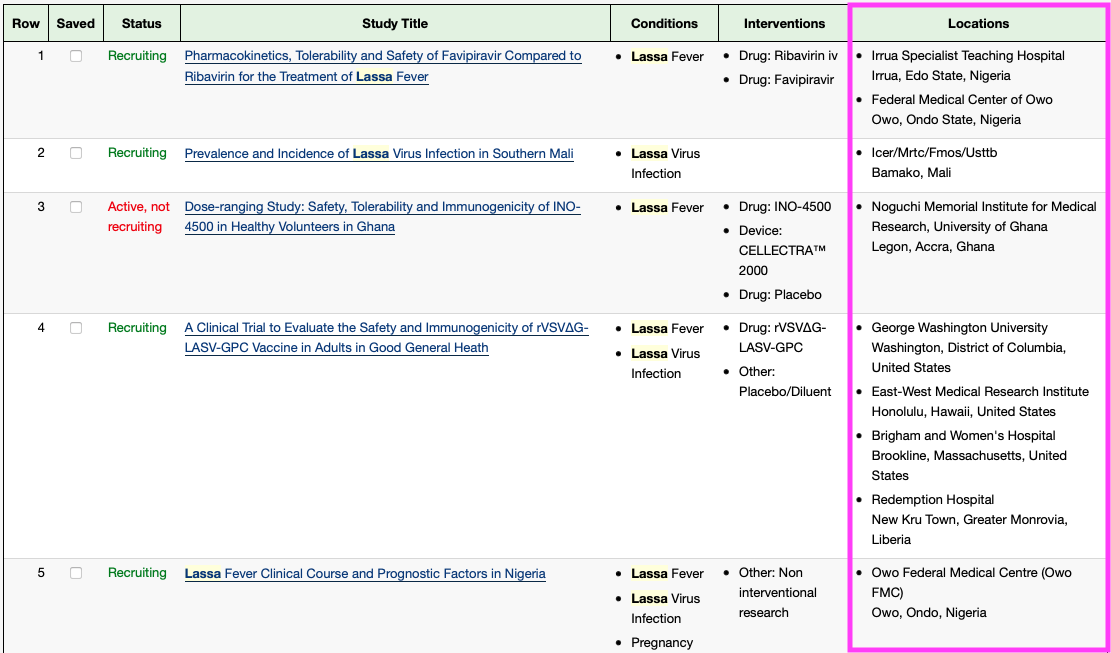
\includegraphics{images/clinicaltrial3.png}

\begin{enumerate}
\def\labelenumi{\arabic{enumi}.}
\setcounter{enumi}{3}
\item
  Click on the first study to start working your way through the information available
\item
  The first information provided is the sponsor -\textgreater{} this information should be added to the Funder -- column in the Activities table
\item
  Information about collaborators can be added to Collaborators column
\end{enumerate}

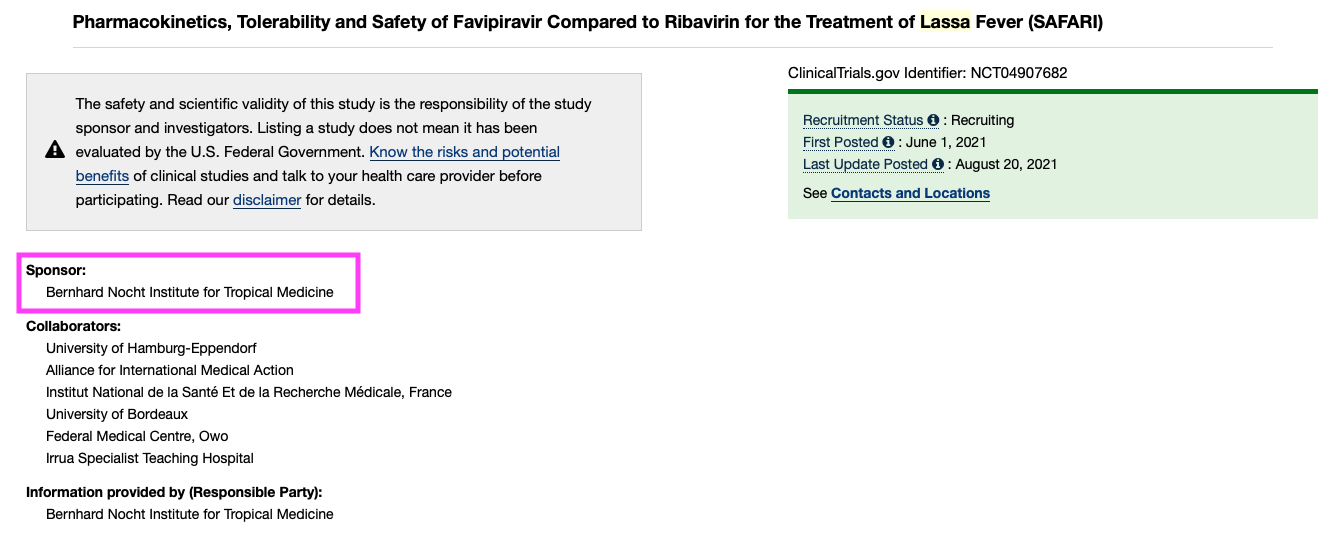
\includegraphics{images/clinicaltrial4.png}

\begin{enumerate}
\def\labelenumi{\arabic{enumi}.}
\setcounter{enumi}{6}
\item
  Staying in the `Study Details'-tab, scroll down to `Study Design'
\item
  This section contains the official title, which should be used as the name for the Activity
\item
  Additionally it contains information about the start and end date, which should be copied into the respective fields in the Activities table
\end{enumerate}

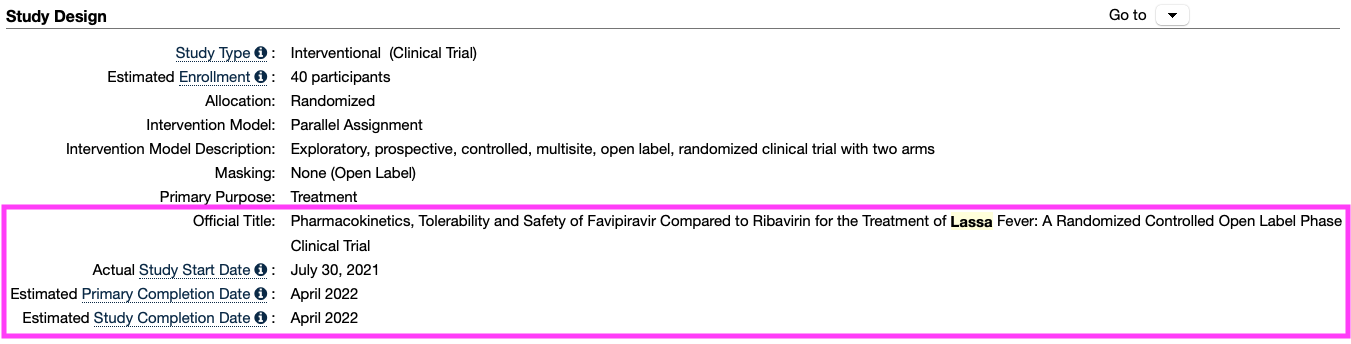
\includegraphics{images/clinicaltrial5.png}

\begin{enumerate}
\def\labelenumi{\arabic{enumi}.}
\setcounter{enumi}{9}
\item
  Scroll further down to `Contact and Locations'
\item
  The information given under contacts should be added to the Researcher column in Airtable
\item
  Switching into the Researcher-table within in Airtable the given contact details should be added to the newly created entries for the involved researchers
\item
  Also the affiliation to a certain institute can be added based on these information as well as the researcher's location -\textgreater{} is it possible to link the Location with the Affiliation so that the location is automatically added based on the information about the institution the researcher is affiliated with?
\item
  Switch back into the Activities table and add information about the Locations to the Activity Location and the Institutions columns
\end{enumerate}


\includegraphics{images/clinicaltrial6.png}

\begin{enumerate}
\def\labelenumi{\arabic{enumi}.}
\setcounter{enumi}{14}
\item
  Scroll up again to the selection of tabs
\item
  Click on the Results tab -\textgreater{} it's worth checking this tab even when it's called No Results Posted as it might still contain links to publications that are affiliated with the study
\item
  These links can be copied into the Published Work column in the Activities table
\end{enumerate}

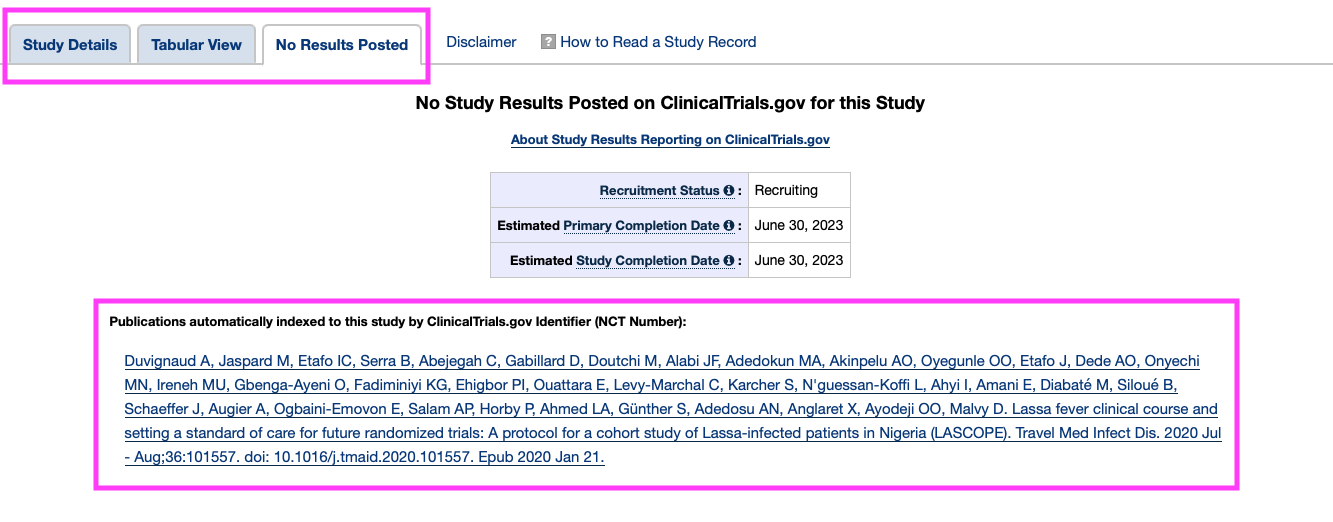
\includegraphics{images/clinicaltrial7.png}

\begin{enumerate}
\def\labelenumi{\arabic{enumi}.}
\setcounter{enumi}{17}
\tightlist
\item
  I also copied the link of the study page on clinicaltrials.gov into the Activity Website column
\end{enumerate}

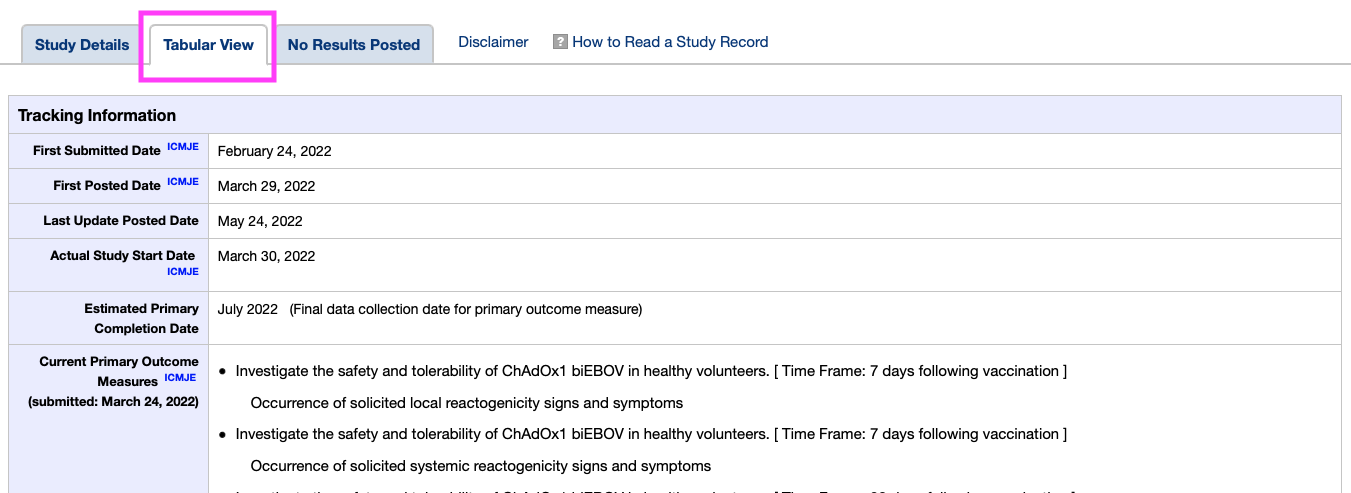
\includegraphics{images/clinicaltrial8.png}

\begin{enumerate}
\def\labelenumi{\arabic{enumi}.}
\setcounter{enumi}{18}
\tightlist
\item
  to determine the Research Field, I had to use my own understanding of the study so I am not sure if this can be automated or rather needs to be done by a database librarian
\end{enumerate}

\hypertarget{update-public-research}{%
\section{Public journal/research databases}\label{update-public-research}}

In order to aid in automation, maintain a list relevant search terms for each topic of interest (stored in the ``Topics'' table in Airtable). Even if the terms are not used for the purposes of developing a search strategy, they can be used by those who are not subject matter experts when collection information on a specific topic

\hypertarget{example-of-a-successful-search}{%
\subsection{Example of a successful search:}\label{example-of-a-successful-search}}

\begin{verbatim}
(zoonoses OR zoonotic disease OR zoonotic illness) and (africa*) and (surveillance OR tracking OR sampling)
\end{verbatim}

The majority of results from this search, when conducted in \href{https://pubmed.ncbi.nlm.nih.gov/}{PubMed}, appeared relevant to the database (based on title/abstract scanning)

\hypertarget{example-of-pubmed-search-for-surveillance-activities-for-brucellosis}{%
\subsection{Example of PubMed search for surveillance activities for Brucellosis:}\label{example-of-pubmed-search-for-surveillance-activities-for-brucellosis}}

\begin{verbatim}
("surveillance"[Title/Abstract] OR "prevalence"[Title/Abstract] OR "monitoring"[Title/Abstract] OR "seropositive"[Title/Abstract] OR "seroprevalence"[Title/Abstract] OR "seroevidence"[Title/Abstract] OR "screened"[Title/Abstract] OR "biosurveillance"[Title/Abstract] OR "sampl*"[Title/Abstract]) AND (brucellosis[Title/Abstract] OR "Brucella melitensis"[Title/Abstract] OR "B. melitensis"[Title/Abstract] OR "Brucella abortus"[Title/Abstract] OR "B. abortus"[Title/Abstract])  
\end{verbatim}

This search yielded a large quantity of results, not all of which were relevant. Manual processes are required to validate results.

Including terms to filter the results based on location were helpful, but still included results not located on the African continent. Search term to filter for African countries:

\begin{verbatim}
(Djibouti[Title/Abstract] OR Seychelles[Title/Abstract] OR DR Congo[Title/Abstract] OR Comoros[Title/Abstract] OR Togo[Title/Abstract] OR Sierra Leone[Title/Abstract] OR Libya[Title/Abstract] OR Tanzania[Title/Abstract] OR South Africa[Title/Abstract] OR Cabo Verde[Title/Abstract] OR Congo[Title/Abstract] OR Kenya[Title/Abstract] OR Liberia[Title/Abstract] OR Central African Republic[Title/Abstract] OR Mauritania[Title/Abstract] OR Uganda[Title/Abstract] OR Algeria[Title/Abstract] OR Sudan[Title/Abstract] OR Morocco[Title/Abstract] OR Eritrea[Title/Abstract] OR Angola[Title/Abstract] OR Mozambique[Title/Abstract] OR Ghana[Title/Abstract] OR Madagascar[Title/Abstract] OR Cameroon[Title/Abstract] OR Côte d'Ivoire[Title/Abstract] OR Namibia[Title/Abstract] OR Niger[Title/Abstract] OR Gambia[Title/Abstract] OR Botswana[Title/Abstract] OR Gabon[Title/Abstract] OR Sao Tome & Principe[Title/Abstract] OR Lesotho[Title/Abstract] OR Burkina Faso[Title/Abstract] OR Nigeria[Title/Abstract] OR Mali[Title/Abstract] OR Guinea-Bissau[Title/Abstract] OR Malawi[Title/Abstract] OR Zambia[Title/Abstract] OR Senegal[Title/Abstract] OR Chad[Title/Abstract] OR Somalia[Title/Abstract] OR Zimbabwe[Title/Abstract] OR Equatorial Guinea[Title/Abstract] OR Guinea[Title/Abstract] OR Rwanda[Title/Abstract] OR Mauritius[Title/Abstract] OR Benin[Title/Abstract] OR Burundi[Title/Abstract] OR Tunisia[Title/Abstract] OR Eswatini[Title/Abstract] OR Ethiopia[Title/Abstract] OR South Sudan[Title/Abstract] OR Egypt[Title/Abstract]) 
\end{verbatim}

From publications, can extract researchers, institutions, funders, activities. Ideally, researchers, institutions, and funders can be extracted automatically as opposed to manually, but scripts would need to be customized for each journal.

\hypertarget{validation-of-results}{%
\subsection{Validation of results}\label{validation-of-results}}

Validation of results can be useful to better understand the overlap between publications and activities and determine the priority of searching through publications vs.~navigating to institution sites directly (or other strategies).

After finding a relevant publication, look at the publication's authors and their respective institutions

Navigate to institutions' sites to search for publications or results from research

Are their activities listed on the site? Are those activities explicitly mentioned in the publications? Etc.

\hypertarget{some-relevant-journalsdatabases}{%
\subsection{Some relevant journals/databases:}\label{some-relevant-journalsdatabases}}

\begin{itemize}
\item
  Zoonoses \& Public Health from Wiley Online Library : \url{https://onlinelibrary.wiley.com/action/doSearch?SeriesKey=18632378\&sortBy=Earliest}
\item
  Journal of Public Health in Africa: \url{https://www.publichealthinafrica.org/jphia/issue/view/30}
\item
  PLoS Journal of Neglected Tropical Diseases: \url{https://journals.plos.org/plosntds/search?filterJournals=PLoSNTD}
\end{itemize}

\hypertarget{update-gepris}{%
\section{GEPRIS}\label{update-gepris}}

\hypertarget{general-information-1}{%
\subsection{General Information:}\label{general-information-1}}

GEPRIS is a database listing all projects funded by the German Research Foundation (German: Deutsche Forschungsgemeinschaft; abbr. DFG) The DFG is a research funding organisation, which functions as a self-governing institution for the promotion of science and research in the Federal Republic Germany. In 2019, the DFG had a funding budget of €3.3 billion.

\hypertarget{how-to-use}{%
\subsection{How to Use:}\label{how-to-use}}

The database can be accessed here: \url{https://gepris.dfg.de/gepris/OCTOPUS?language=en\&task=showSearchSimple}

This link should directly lead to the English version of the website, otherwise the language can be changed by clicking on English in the top right corner.

\begin{itemize}
\item
  In the database one can search for Projects, People, or Institutions -- for our purpose the project option is the most relevant
\item
  One can either search for keywords or filter for different criteria -- for a systematic approach I found using the filtering options easier than going through all our
\end{itemize}

\begin{enumerate}
\def\labelenumi{\arabic{enumi}.}
\item
  On the search start site stay in the Projects tab.
\item
  Click on Show extended search.
\item
  Under Subject Area select one of the following:

  \begin{itemize}
  \item
    Agriculture, Forestry and Veterinary Medicine
  \item
    Basic Research in Biology and Medicine
  \item
    Medicine
  \item
    Microbiology, Virology, and Immunology
  \item
    Social Sciences
  \item
    Water Research
  \item
    Zoology
  \end{itemize}
\end{enumerate}

\textbf{Note:} After working through all these subject areas, any relevant project in the field of One Health should be picked up by the searches

\begin{enumerate}
\def\labelenumi{\arabic{enumi}.}
\setcounter{enumi}{3}
\item
  Leave everything under DFG Programme as it is
\item
  Move on to Funding and change Status to Current
\item
  Move on to International and change Continent to Africa
\item
  Click on Find
\item
  Read through the project titles on the results page to identify relevant projects
\item
  Import all the relevant project information (as highlighted on the screenshots) into the Africa CDC database
\end{enumerate}

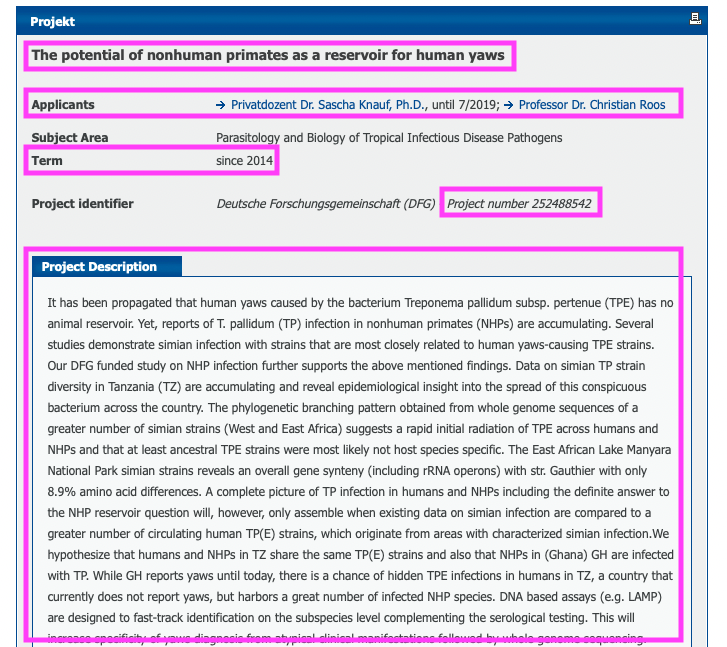
\includegraphics{images/gepris1.png}
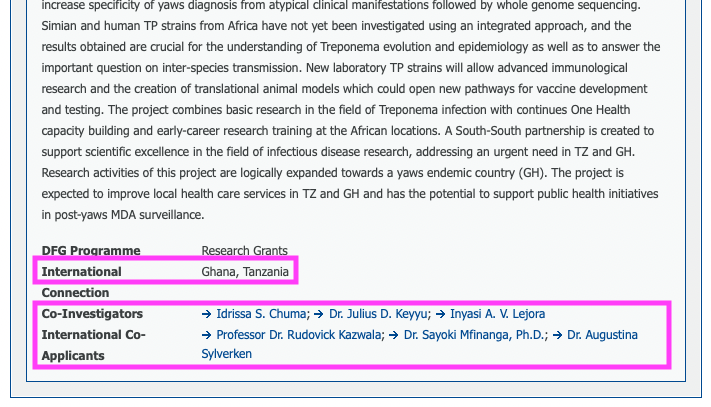
\includegraphics{images/gepris2.png}

\begin{enumerate}
\def\labelenumi{\arabic{enumi}.}
\setcounter{enumi}{9}
\tightlist
\item
  To identify the research institutes that are involved in the project one has to click on the researchers names and extract that information from their profile (their affiliation with a research institute is listed there)
\end{enumerate}

\hypertarget{positive-aspects-of-this-source}{%
\subsection{Positive aspects of this source:}\label{positive-aspects-of-this-source}}

The filtering options allow to filter for several criteria which are crucial for the relevance of a project to our database. That removes a lot of irrelevant projects from the results pages. The project pages list almost all the information we are interested in.

\hypertarget{downsides-of-this-source}{%
\subsection{Downsides of this source:}\label{downsides-of-this-source}}

The project page doesn't list the anticipated end date of a project.

One has to click on the link to the researcher's profile to identify the participating organisations.

Even using all the different filtering options not all resulting hits are relevant for our database, so I don't think the process can be fully automated or at least requires a subsequent manual validation or clean up step to remove irrelevant projects.

\hypertarget{update-edctp}{%
\section{EDCTP}\label{update-edctp}}

\hypertarget{general-information-2}{%
\subsection{General Information}\label{general-information-2}}

The European \& Developing Countries Clinical Trials Partnership (EDCTP) is a non-profit organisation with a European office in The Hague, The Netherlands and an African office in Cape Town, South Africa. EDCTP is a partnership between European Union (EU), Norway, Switzerland, and African countries to accelerate the development of new clinical interventions such as drugs, vaccines, microbicides, and diagnostics against poverty-related diseases in Africa. The organisation supports clinical trials, capacity strengthening and networking in Africa and Europe. Funding comes from the EU, member states, pharmaceutical industry and private organisations and charities like The Wellcome Trust and The Bill \& Melinda Gates foundation.

\textbf{Note:} Since funding comes from several sources that we also list as sources for populating the database such as the European Union (European Commission), The Wellcome Trust and The Bill \& Melinda Gates Foundation, there is the possibility that downloading project information from all these sources into our database could lead to duplicate entries. I created a column in the Actvities table for the Project ID, as this might be helpful to identify duplicates and remove them automatically.

\hypertarget{how-to-use-1}{%
\subsection{How to use:}\label{how-to-use-1}}

The database of funded project can be accessed here: \url{https://www.edctp.org/edctp2-project-portal/}

There is the option to download the list of projects as a PDF, CSV or XLXS file. Personally, I did not find that helpful for manually adding projects to the database, but it might be useful for an automated process.

\begin{enumerate}
\def\labelenumi{\arabic{enumi}.}
\item
  Go to Status of Project and select the filter Active
\item
  Go to Classification and select one of the following filters:

  \begin{itemize}
  \tightlist
  \item
    Co-Infections
  \item
    COVID-19
  \item
    Cysticercosis/Taeniasis\\
  \item
    Diagnostics
  \item
    Diarrhoeal Diseases
  \item
    Drugs
  \item
    Emerging Infections, incl.~Ebola, Lassa
  \item
    Epidemiology
  \item
    HIV
  \item
    Human African trypanosomiasis (sleeping sickness)\\
  \item
    Implementation Research\\
  \item
    Leishmaniases
  \item
    Leprosy (Hansen disease)
  \item
    Lower respiratory infections\\
  \item
    Lymphatic filariasis
  \item
    Malaria
  \item
    Microbicides
  \item
    Onchocerciasis (river blindness)
  \item
    Rabies
  \item
    Schistosomiasis
  \item
    Soil-transmitted helminthiasis\\
  \item
    Social Science
  \item
    Tuberculosis
  \item
    Vaccines
  \item
    Yaws
  \item
    Yellow Fever
  \end{itemize}
\end{enumerate}

\textbf{Note:} Only one Classification at a time can be selected

\begin{enumerate}
\def\labelenumi{\arabic{enumi}.}
\setcounter{enumi}{2}
\item
  Once one Classification was selected click on search
\item
  Change from Show Map to Show List -\textgreater{} this makes it easier to systematically look through the projects
\item
  On the results list you can see the location of the coordinating organisation, but even if it is not in an African country, it is worth checking the project details for the Participating Organisations. So read the project title and decide whether this could be a relevant project, if so, click on View details
\end{enumerate}

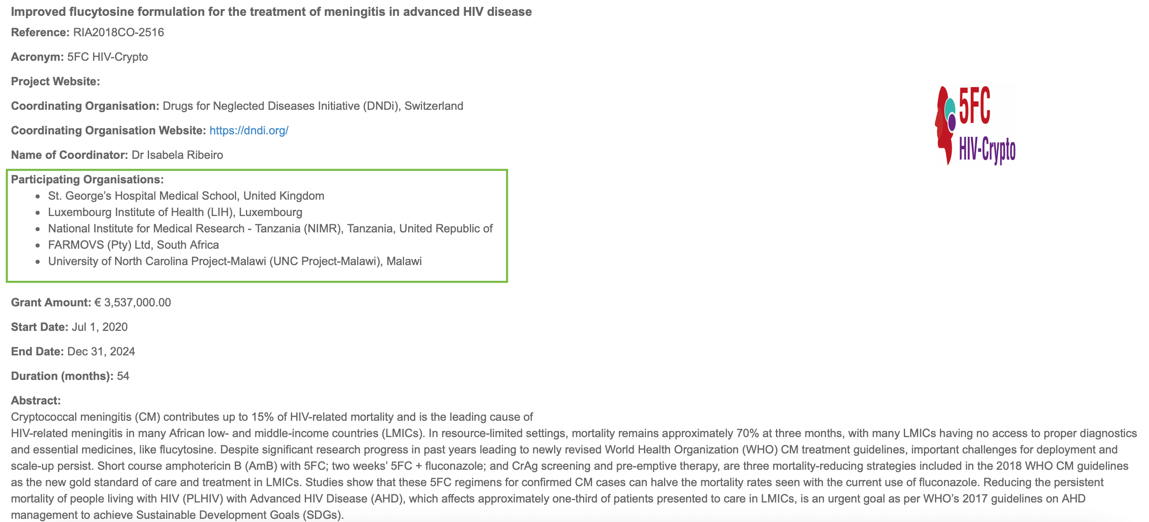
\includegraphics{images/edctp1.png}

\begin{enumerate}
\def\labelenumi{\arabic{enumi}.}
\setcounter{enumi}{5}
\tightlist
\item
  Check the Participating Organisations first to decide whether the project is relevant to our database:
\end{enumerate}

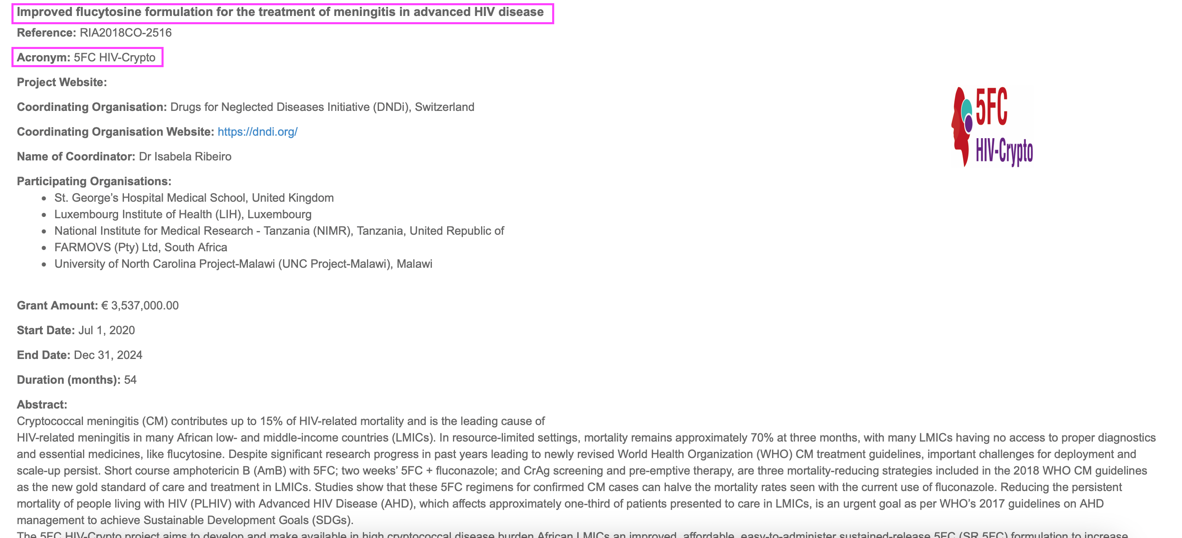
\includegraphics{images/edctp2.png}

\begin{enumerate}
\def\labelenumi{\arabic{enumi}.}
\setcounter{enumi}{6}
\item
  If the project is relevant use the Project Name + Acronym for the Activity Column
\item
  Transfer all the relevant information to our database, including Project ID, Start and End date, Participating Organisations and corresponding locations, Project Website, Coordinating Organisation and Coordinating Researcher
\item
  Tag the project with the correct keywords in the Activity Type, Activity Outputs, Target Species, Topic, and Research Field columns based on your understanding of the project abstract
\end{enumerate}

\hypertarget{benefits-of-this-source}{%
\subsection{Benefits of this Source:}\label{benefits-of-this-source}}

The projects can be easily filtered for currently active projects.

The EDCTP is specifically focused on projects in Africa or Europe with African collaborators so most projects fulfil at least one of our selection criteria

A lot of the projects (not all) are also topic-wise relevant for our database

The database lists most of the information that we are interested in for our database

\hypertarget{shortcomings-of-this-source}{%
\subsection{Shortcomings of this source:}\label{shortcomings-of-this-source}}

Only one disease/topic can be selected at a time so sequential searches are necessary

Project details only list the Coordinating researcher but no other lead researchers at the participating organisations

\hypertarget{survey}{%
\chapter{Survey}\label{survey}}

  \bibliography{book.bib}

\end{document}
